\documentclass{article}

% Language setting Replace `english' with e.g. `spanish' to change the document
% language
\usepackage[english]{babel}
\usepackage{caption}
\usepackage{subcaption}
\usepackage{makecell}
\usepackage[toc,page]{appendix}
\setlength{\marginparwidth}{2cm}
\usepackage{todonotes}
\usepackage{soul}
\usepackage{pdflscape}


% Set page size and margins Replace `letterpaper' with `a4paper' for UK/EU
% standard size
\usepackage[letterpaper,top=2cm,bottom=2cm,left=3cm,right=3cm,marginparwidth=1.75cm]{geometry}

% Useful packages
\usepackage{amsmath}
\usepackage{amsfonts}
\usepackage{amssymb}
\usepackage{graphicx}
\usepackage{xspace}
\usepackage{xcolor}% http://ctan.org/pkg/xcolor
\usepackage{hyperref}
\usepackage{colortbl}
\usepackage{dsfont}

\setlength{\marginparwidth}{2cm}
\usepackage{todonotes}

\newcommand{\TODO}[1]{\color{red}\textsc{TODO:} #1\color{black}\xspace}
\newcommand{\TG}[1]{\color{blue}\textsc{From Tristan:} #1\color{black}\xspace}
\newcommand{\fmriprep}{fMRIPrep\xspace}
\newcommand{\fwhm}{\textsc{FWHM}}

\newcommand\Mark[2][8.4]{%
  \rlap{\tikz[baseline=(current bounding box.south)]{
        \shade[left color=\color{red}, right color=\color{green}, middle color=\color{yellow}]
               (0,0) rectangle ++(#1*#2/100,0.3);}%
  }%
}

% Cluster failure: Why fMRI inferences for spatial extent have inflated
% false-positive https://www.pnas.org/doi/pdf/10.1073/pnas.1602413113

\title{Non-regression tests for structural MRI analysis: towards a numerical uncertainty approach}
\author{Yohan Chatelain, Loic Tetrel, Christopher J. Markiewicz, Gregory Kiar,\\ Oscar Esteban,  Pierre Bellec, Tristan Glatard}

\begin{document}
\maketitle

\begin{abstract}
    Target: PLOS ONE, Frontiers in Neuroinformatics,  IEEE Transactions on
    Software Engineering. \url{https://www.computer.org/csdl/journal/ts}
\end{abstract}

\section{Introduction}

The need for and requirements of long-term support of neuroimaging software:
\begin{itemize}
    \item Span over several years. Software updates are unavoidable (security
          updates, EOL, etc).
    \item Neuroimaging software can be unstable, variation across packages are
          significant -> therefore need to be tested
    \item for instance: fmriprep LTS project
\end{itemize}

Non-regression testing in neuroimaging:
\begin{itemize}
    \item Testing is difficult because (1) there is no reference (ground truth),
          (2) as in many other contexts, defining an acceptable tolerance (variation
          bounds) is difficult.
    \item there are methods to evaluate software in the absence of ground truth
          (simulation, phantoms, ex-vivo) but they all have their own limitations and
          they don't allow for the definition of acceptable variation bounds.
    \item There are no widely accepted bounds of variation around any reference.
          Variation bounds may be defined specifically for each application (e.g.,
          from the measured effect on the F1 score of a classifier), but the stability
          of pre-processing must be guaranteed independently of any particular
          application.
    \item Our approach is to define a reference result and acceptable variation
          bounds around this reference from the numerical uncertainty measured in the
          reference software version. Using a set of representative datasets.
    \item Numerical variability is a critical property of scientific data
          analyses [ref Greg]. Numerical uncertainty may capture the variation that
          would be experienced by users when using the software tool in different
          environments including different hardware architectures and software stacks.
    \item We build on previous evaluations of numerical variability in
          neuroimaging: ref greg \& ali
    \item We measure this uncertainty using random rounding (references,
          summarize principle).
\end{itemize}

\begin{figure}

\end{figure}

The same method could be applied to other domains where ground truth is not
available or acceptable variation bounds cannot be easily defined.

Mention that based on previous results, libmath explains a large amount of
numerical variability observed across OS differences. Explain GNU libmath.

Define LTS as an arbitrary reference version of fMRIPrep.

Correcting for multiple comparisons is a challenge. Refer to main methods used
in neuroimaging. Explain that we have images, voxels, etc

fMRIPrep is a functional magnetic resonance imaging (fMRI) data preprocessing
pipeline designed to provide an easily accessible, state-of-the-art interface
that is robust to variations in scan acquisition protocols and that requires
minimal user input, while providing easily interpretable and comprehensive error
and output reporting. It performs basic processing steps (coregistration,
normalization, unwarping, noise component extraction, segmentation,
skullstripping etc.) to provide outputs that can be easily submitted to a
variety of group level analyses, including task-based or resting-state fMRI,
graph theory measures, surface or volume-based statistics, etc. We focused our
study on the structural analysis pipeline of fMRIPrep for simplicity.




Paper goal:
\begin{itemize}
    %\item G1: To measure the numerical variability of MRI structural analysis
    \item G1: Build and evaluate a non-regression test for structural MRI
          analysis. The baseline is LTS, using numerical variability as an acceptable
          variation bound.
          %\item G2: To verify that statistical test captures unstable
          %computations
\end{itemize}


% BOnferonni 0.75 for inter FDR-BY 0.8 for all- exclude / include

\section{Non-regression test design}

% \subsection{Logic of the test}

The non-regression test checks whether results produced by an updated version of
fMRIPrep or obtained in a different execution environment deviate from the
reference fMRIPrep LTS results. We estimate the distribution of reference
results by introducing numerical perturbations in fMRIPrep LTS in a way that
mimics variability resulting from changes in the execution environment.  For
each voxel $x_i$ in each test image, we perform a z-test for the tested fMRIPrep
version (non-perturbed, IEEE result) using the mean and standard deviation
estimated from $n$ perturbed results. The test computes a p-value under the null
hypothesis $H_{0,i}$ that the value produced by the tested fMRIPrep version
belongs to the reference distribution:
\begin{equation}
    \label{eqn:pval}
    p_i(z_i) = 2 \left(1-\Phi(z_i)\right),
\end{equation}
where $\Phi$ is the cumulative distribution function of the normal centered
Gaussian and:
\begin{equation*}
    z_i = \frac{x_i-\hat \mu_i}{\hat \sigma_i},
\end{equation*}
where $x_i$, $i < v$ is the voxel intensity obtained after pre-processing the
output of the tested fMRIPrep version, $v$ is the number of voxels, and $\hat
    \mu_i$ and $\hat \sigma_i$ are the mean and standard deviation voxel intensity
estimated from the $n$ perturbed results. $H_{0,i}$ is rejected when $p_i$ is
lower than a threshold $\alpha$ from which the confidence level of the test
(1-$\alpha$)\% is also defined. The z-test assumes that perturbed voxel
intensities are normally distributed. To capture anatomical variability, we
perform this test on a representative set of brain structural images.

\TG{add a table of notations}

\begin{figure}
    \centering
    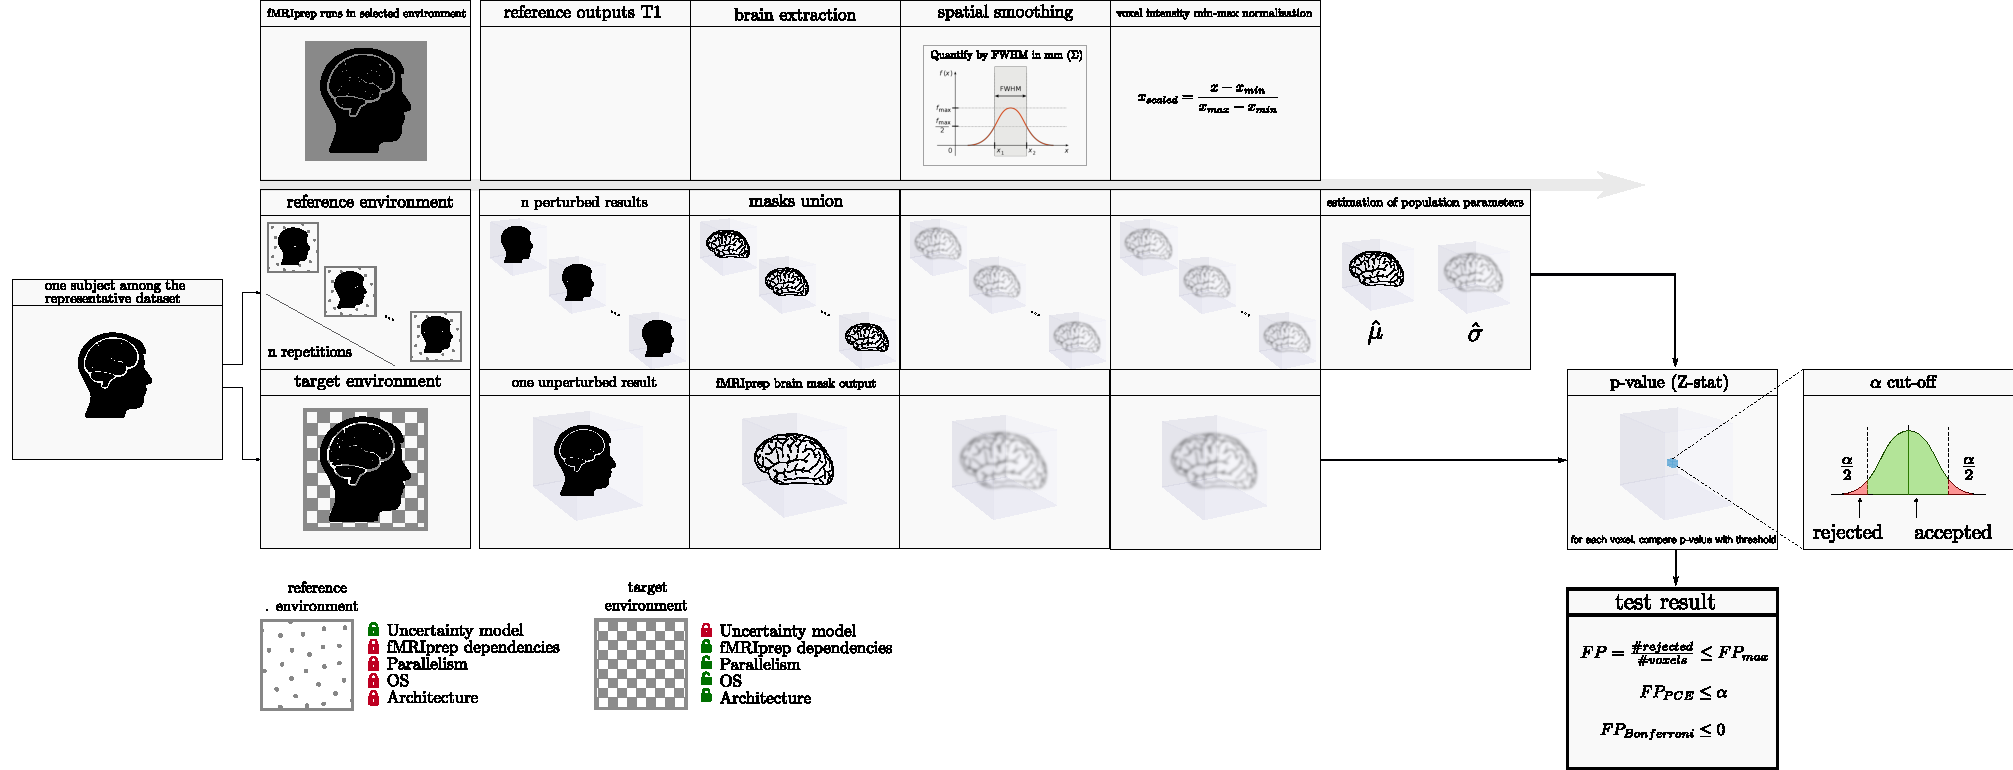
\includegraphics[width=\linewidth]{figures/stat_test_procedure.pdf}
    \caption{Test workflow.}
    \label{fig:test_workflow}
\end{figure}

\subsection{Numerical variability estimation}

To estimate the distribution of reference fMRIPrep results across execution
environments and compute $\hat \mu$ and $\hat \sigma$ (Equation~\ref{eqn:pval}), we
sample results distributions by applying three types of numerical perturbations
to the computations: (1) Random Rounding (RR), which randomly rounds function
outputs in the GNU libmath, (2) Random Seed (RS), which varies the random seed
used in fMRIPrep, and (3) Random Rounding + Random Seed (RR+RS), which applies
both previous perturbations.

Random Rounding (RR) consists in rounding the exact result of a floating-point
arithmetic operation toward the previous or next floating-point number with
equal probability~\cite{forsythe1959reprint}. RR is equivalent to applying
Monte-Carlo Arithmetic (MCA) to double-precision numbers with a virtual
precision of 53 bits and to single-precision numbers with a virtual precision of
24 bits, which was shown to accurately simulate the effect of operating system
updates on the structural pre-processing pipelines of the Human Connectome
Project (HCP) when applied to GNU libmath~\cite{salari2021accurate}. Structural
HCP pipelines consist of tools assembled from the FSL~\cite{jenkinson2012fsl}
and Freesurfer~\cite{fischl2012freesurfer} toolboxes, which makes them
conceptually very similar to the structural fMRIPrep pipeline.

RR is rigorously implemented in several tools including
CADNA~\cite{jezequel2008cadna}, Verrou~\cite{fevotte2016verrou}, and
Verificarlo~\cite{denis2016verificarlo}. However, these tools incur substantial
performance overheads which makes them difficult to use with a compute-intensive
pipeline such as fMRIPrep. In addition, only Verrou supports RR instrumentation
of GNU libmath~\cite{fevotte2019debugging}, and it does so by relying on
quadruple precision, which is not scalable to the entire fMRIPrep pipeline.
Therefore, we implemented a fast, approximate RR method by randomly adding or
removing 1 ulp (unit in the last place) to the outputs of GNU libmath functions.
Our implementation is available on \href{https://github.com/verificarlo/fuzzy}{GitHub}.
It only
approximates RR as it applies the random perturbation to an already rounded
result instead of to the exact result as done in rigorous implementations. In
practice, computing the exact result returned by GNU libmath functions is too
expensive for our use case.

Random Seeds (RS) define pseudo-random number sequences involved in various
numerical procedures such as algorithm initialization (e.g., in k-means) or
stochastic optimization (e.g., stochastic gradient descent). In fMRIPrep, random
seeds are used in skull stripping, ANTs on linear registration, \TODO{to check}.
\TODO{https://github.com/ANTsX/ANTs/wiki/Anatomy-of-an-antsRegistration-call}
fMRIPrep provides an interface to set the random seed for all the pipeline
components except skull stripping, which we used in our experiments. RS and RR
trigger different types of variability. RR can be applied transparently to any
application while RS is more specific to the type of analysis. Conversely, RR
incurs a substantial performance overhead whereas RS does not.

\subsection{fMRIprep results preprocessing}

The non-regression test applies to the main structural derivative produced by
\fmriprep: the T1 image corrected for intensity non-uniformity using
\texttt{N4BiasFieldCorrection} from \texttt{ANTS} and transformed to template
space using
\texttt{antsRegistration}, named \texttt{desc-preproc\_T1w} in the \fmriprep
outputs and $X_k$ ($k < n$) in the remainder of this paper. In addition to the
pre-processed T1 image $X_k$, \fmriprep produces a brain mask ($B_k$), a
segmentation into grey matter, white matter and cerebro-spinal fluid tissues, as
well as probability maps for each of these tissues.

Before computing the p-values in Equation~\ref{eqn:pval}, we apply the following
pre-processing steps to $X_k$: brain masking, smoothing, and intensity
normalization. For brain masking, we mask $X_k$ with the union of the brain
masks produced across all perturbed results. We use the union of the brain masks
rather than their intersection to capture variability across $B_k$ masks. For
smoothing, we apply a spatial 3D Gaussian smoothing kernel with Full-Width at Half
Maximum (\fwhm) ranging from 0~mm to 20~mm. For intensity normalization, we apply
a min-max scaling to the smoothed intensities to scale them to [0,1].

\subsection{Handling multiple comparisons}

Handling multiple comparisons is a critical component of statistical testing in
neuroimaging given the high number of voxels tested for each 3D structural
image---typically more than 10 million~\cite{NICHOLS2007246}. The non-regression
test defined in Equation~\ref{eqn:pval} consists of independent z-tests performed
for each of the $v$ voxels of each test image, resulting in a set of $v$
p-values $p_i$, $i < v$. We corrected for multiple comparisons by adjusting the p-value
threshold. We use the classical Bonferroni correction that simply divides
$\alpha$ by the number of multiple comparisons performed. As a result, the
tested \fmriprep result is considered part of the reference distribution iif:
\begin{equation}
    \label{eq:bonferroni}
    \forall i, \quad i < v, \quad p_i < \frac{\alpha}{v}.
\end{equation}

% \begin{table}[] \centering \begin{tabular}{c|c|c|c} & Negatives & Positives &
%     \\
%          True noise  & $V_{0N}$ & $\mathbf{V_{0P}}$ & $v_0$ \\
%          True signal & $V_{1N}$ & $V_{1P}$ & $v_1$ \\
%                      & $V_N$    & ${V_P}$    & $v$ \end{tabular}
%     \caption{Cross-classification of all $v$ voxels in an image.}
%     \label{tab:cross-classification-fp} \end{table}


\subsection*{Numerical variability measure}

We compute the significant bits $\hat{s}$ with probability $p$ and confidence $1-\alpha$
using the \texttt{significant\_digits} package
v0.1.2 available at \url{https://github.com/verificarlo/significantdigits} that
implements the Centered Normality Hypothesis approach described in~\cite{sohier2021confidence}:

\[
    \hat{s} = -\log_2 \left| \frac{\hat{\sigma}}{\hat{\mu}} \right| - \delta(n, \alpha, p)
\]
where $\hat{\sigma}$ and $\hat{\mu}$ are the voxelwise average and standard
deviation over the $X_i$ perturbed results ($i \leq n$),
and
\[
    \delta(n, \alpha, p) =
    \left[
        \frac{1}{2} \log_2 \left( \frac{n-1}{\chi^2_{1-\alpha/2}} \right) +
        \log_2 \left( \Phi^{-1} \left( \frac{p+1}{2} \right) \right)
        \right]
\]
is a penalty value to have an estimator of $s$ with a probability $p$ and a confidence level $1-\alpha$ for
a sample size $n$. $\Phi^{-1}$ is the inverse cumulative distribution of the standard normal distribution
and $\chi^2$ is the Chi-2 distribution with n-1 degrees of freedom.

\subsection{Datasets}

We selected eight test subjects from sub-datasets in OpenNeuro, representing a
diversity of age, sex, and study designs. The datasets include a motion study
with children (ds000256), a long-term memory study with young adults (ds001748),
and a motor process study with adults (ds002338). In addition, two sub-datasets
involve steps of the pipeline that can affect its reproducibility, namely
different field maps (ds001600) and non-structural images (ds001771).
Table~\ref{table:dataset_info} lists the dimension, voxels resolution, age and sex of each
subject in the dataset.

\begin{table}
    \begin{center}
        \begin{tabular}{c|c|l|c|c|c|c|c}
            Index & Dataset  & Subject     & Dimension ($x,y,z$)         & Voxel resolution $mm^3$ ($x,y,z$) & Data type & Age  & Sex \\
            \hline
            1     & ds001600 & sub-1       & $176 \times 256 \times 256$ & $1.0 \times 1.0 \times 1.0$       & int16     & -    & -   \\
            2     & ds001771 & sub-36      & $256 \times 320 \times 320$ & $0.8 \times 0.8 \times 0.8$       & int16     & 22   & F   \\
            3     & ds000256 & sub-CTS201  & $256 \times 256 \times 256$ & $1.0 \times 1.0 \times 1.0$       & int16     & 8.68 & M   \\
            4     & ds000256 & sub-CTS210  & $224 \times 256 \times 256$ & $0.8 \times 0.8 \times 0.8$       & int16     & 7.63 & F   \\
            5     & ds001748 & sub-adult15 & $176 \times 240 \times 256$ & $1.0 \times 1.0 \times 1.0$       & float32   & 21   & M   \\
            6     & ds001748 & sub-adult16 & $176 \times 240 \times 256$ & $1.0 \times 1.0 \times 1.0$       & float32   & 21   & F   \\
            7     & ds002338 & sub-xp201   & $176 \times 512 \times 512$ & $1.0 \times 0.5 \times 0.5$       & int16     & 41   & F   \\
            8     & ds002338 & sub-xp207   & $176 \times 512 \times 512$ & $1.0 \times 0.5 \times 0.5$       & int16     & 39   & M   \\
        \end{tabular}
    \end{center}
    \caption{Dimension, voxels resolutions, age and sex of each subject in the dataset.}
    \label{table:dataset_info}
\end{table}


% \TG{report on resolution and data types}

% \begin{itemize}
%     \item \st{Describe Openneuro project}
%     \item \st{Describe each dataset}
% \end{itemize}

\subsection{Computing infrastructure}

We processed the dataset using the Narval cluster managed by Calcul Qu\'ebec and
Compute Canada. With our job submission parameters, we could access 1,145
computing nodes with 64 cores per node and 2 $\times$ AMD Rome 7532 @ 2.40 GHz
256M cache L3. We executed \fmriprep in a Singularity container built from a
Docker image available on dockerhub \texttt{yohanchatelain/fmriprep-fuzzy:20.2.1}.
The container image used Ubuntu \texttt{16.04.6 LTS}, GNU
libc/libmath \texttt{2.23}, kernel \texttt{4.18.0-372.19.1}
\texttt{.el8\_6.x86\_64}, and fMRIPrep version \texttt{20.2.1}. We disabled
multi-threading in fMRIPrep, fixed the random seed for skull stripping as well
as in fMRIPrep (RR condition only), and verified that in these conditions
fMRIPrep results were bit-to-bit reproducible.

\section{Results}

We computed 30 perturbed results for each of the 8 subjects and each of the 3
perturbations (RR, RS, RR+RS). We also computed an unperturbed IEEE
result for each subject using the random seed (42) as RR. For each perturbation we
measured the uncertainty of fMRIPrep in terms of significant bits, and we
built the non-regression test using different values of FWHM smoothing and confidence level.

\subsection{Measured uncertainty}

Overall, the three types of perturbations (RR, RS, RR+RS) created uncertainties
of comparable magnitude (Figure~\ref{fig:significant-digits}). The measured
uncertainty is high, with mean significant bits ranging from 2 bits to 10 bits
out of the 12 bits available in the data. Numerically, \fmriprep appears to be
highly sensitive to the numerical and random seed perturbation. We also observe
substantial discrepancies among subjects. For a given smoothing kernel size, the
number of significant bits frequently varies in the ratio of 1 to 3 among
subjects. Overall, smoothing tends to reduce numerical uncertainty, however,
this behavior is in general not monotonous and varies across subjects.

The uncertainty measured across perturbed samples showed regional variations
compatible with anatomical features (Figure~\ref{fig:uncertainty-maps}). In
particular, uncertainty was maximal at the border of the brain mask, and it was
overall higher in the gray matter than in the white matter. This is consistent
with previous observations of numerical uncertainty in structural brain image
analysis~\cite{salari2021accurate}. In addition, uncertainty was also maximal in
some cortical regions, suggesting that non-linear registration may be unstable
in these regions. Our non-regression test will therefore be more tolerant in
these regions.


\begin{figure}
    \centering
    \includegraphics[width=\linewidth]{figures/stats.pdf}
    \caption{Voxel-wise means of mean, standard deviation and significant bits
        measured across n=30 perturbed samples for 3 types of perturbations and 8
        subjects. For each subject, we computed statistics in the union of the brain
        masks among n=30 perturbed samples.}
    \label{fig:significant-digits}
\end{figure}

\begin{landscape}
    \begin{figure}

        \vspace*{-2cm}
        \centering
        %% sub 1
        \begin{subfigure}[b][][c]{0.01\paperwidth} 1 \vspace*{-45pt} \end{subfigure}
        \begin{subfigure}[t]{0.2\paperheight}
            \centering
            IEEE (T1 intensity)
            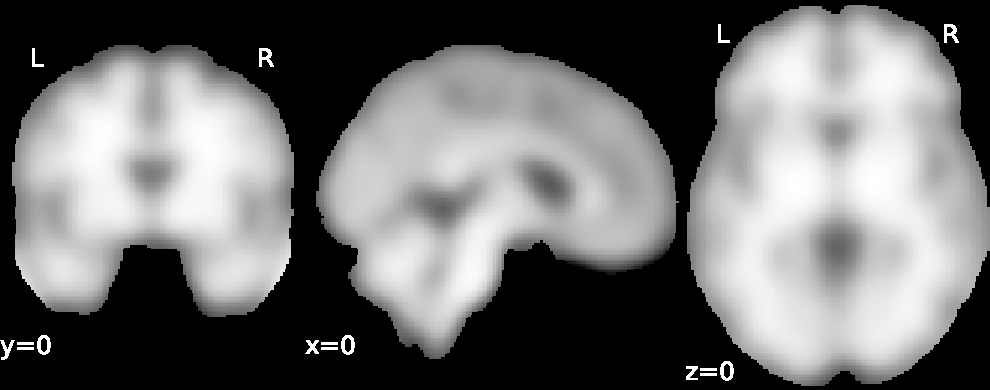
\includegraphics[width=\textwidth]{figures/sig/15mm/ieee_ds001600_sub-1.pdf}
        \end{subfigure}
        \begin{subfigure}[t]{0.2\paperheight}
            \centering
            RR (significant bits)
            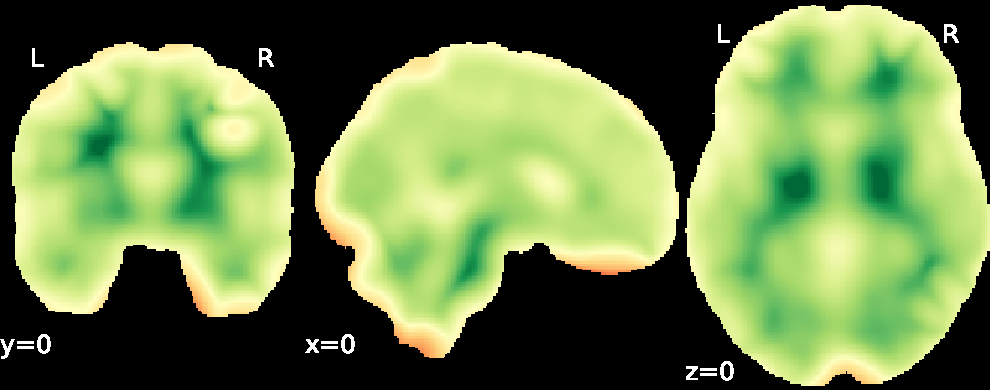
\includegraphics[width=\textwidth]{figures/sig/15mm/rr_ds001600_sub-1_sig.pdf}
        \end{subfigure}
        \begin{subfigure}[t]{0.2\paperheight}
            \centering
            RS (significant bits)
            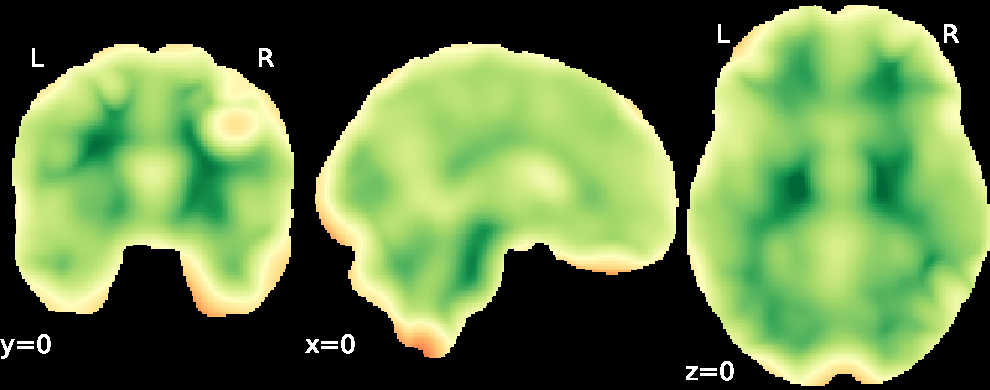
\includegraphics[width=\textwidth]{figures/sig/15mm/rs_ds001600_sub-1_sig.pdf}
        \end{subfigure}
        \begin{subfigure}[t]{0.2\paperheight}
            \centering
            RS (significant bits)
            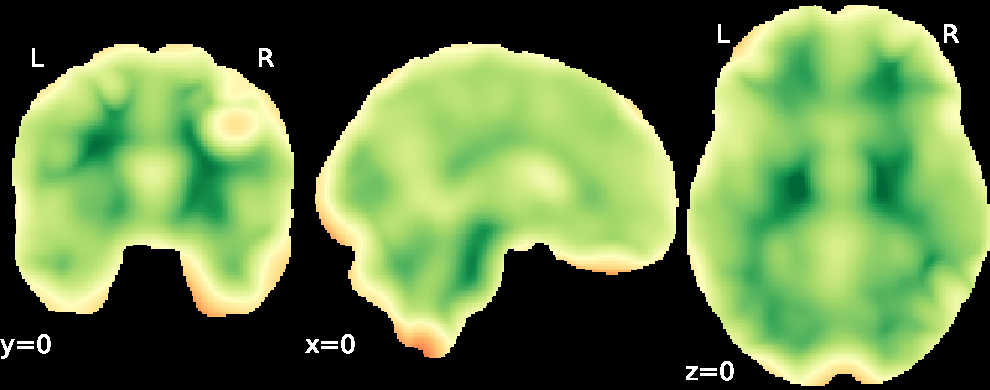
\includegraphics[width=\textwidth]{figures/sig/15mm/rs_ds001600_sub-1_sig.pdf}
        \end{subfigure} \\
        %% sub 2
        \begin{subfigure}[b][][c]{0.01\paperwidth} 2 \vspace*{15pt} \end{subfigure}
        \begin{subfigure}[t]{0.2\paperheight}
            \centering
            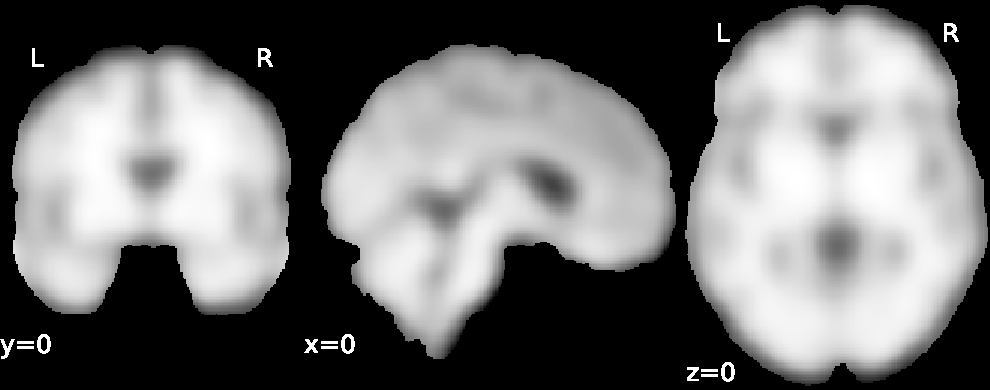
\includegraphics[width=\textwidth]{figures/sig/15mm/ieee_ds001771_sub-36.pdf}
        \end{subfigure}
        \begin{subfigure}[t]{0.2\paperheight}
            \centering
            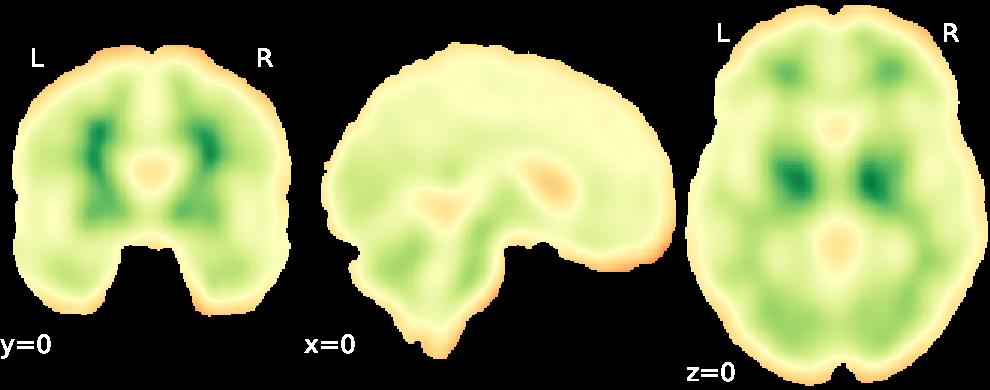
\includegraphics[width=\textwidth]{figures/sig/15mm/rr_ds001771_sub-36_sig.pdf}
        \end{subfigure}
        \begin{subfigure}[t]{0.2\paperheight}
            \centering
            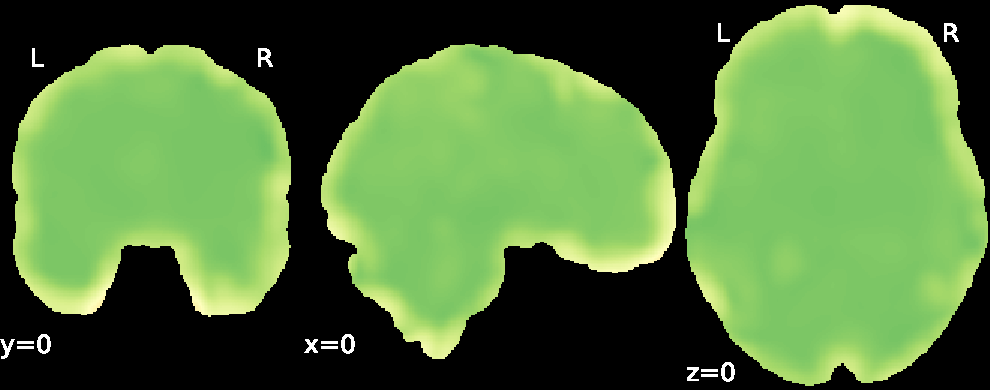
\includegraphics[width=\textwidth]{figures/sig/15mm/rs_ds001771_sub-36_sig.pdf}
        \end{subfigure}
        \begin{subfigure}[t]{0.2\paperheight}
            \centering
            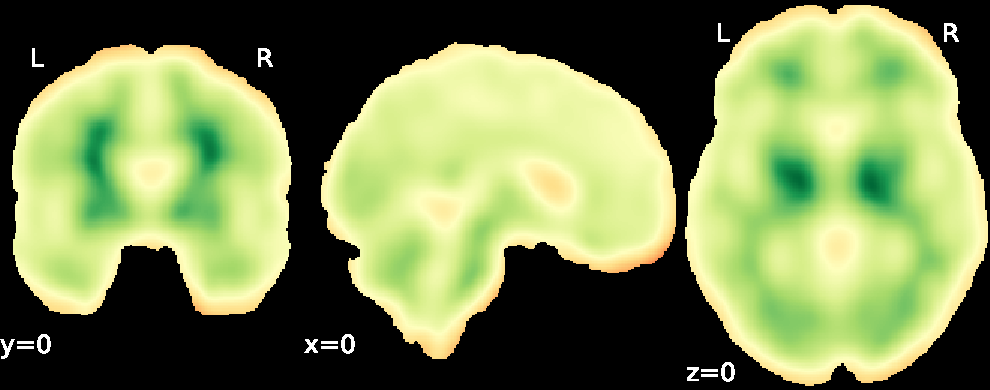
\includegraphics[width=\textwidth]{figures/sig/15mm/rr.rs_ds001771_sub-36_sig.pdf}
        \end{subfigure} \\
        %% sub 3
        \begin{subfigure}[b][][c]{0.01\paperwidth} 3 \vspace*{15pt} \end{subfigure}
        \begin{subfigure}[t]{0.2\paperheight}
            \centering
            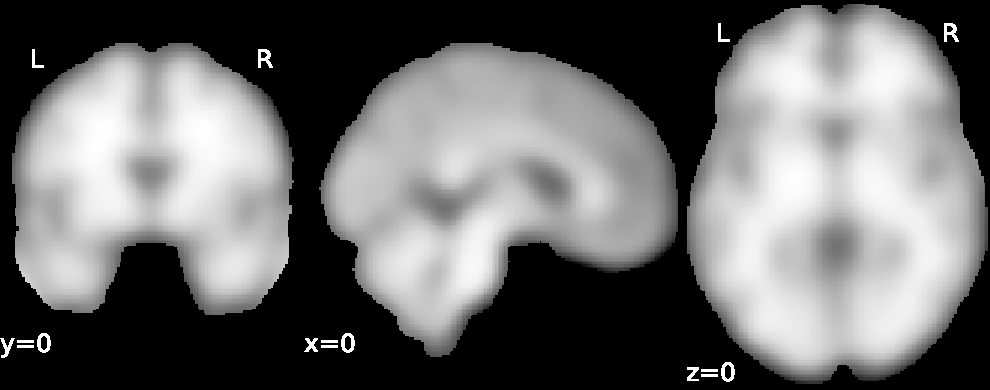
\includegraphics[width=\textwidth]{figures/sig/15mm/ieee_ds000256_sub-CTS201.pdf}
        \end{subfigure}
        \begin{subfigure}[t]{0.2\paperheight}
            \centering
            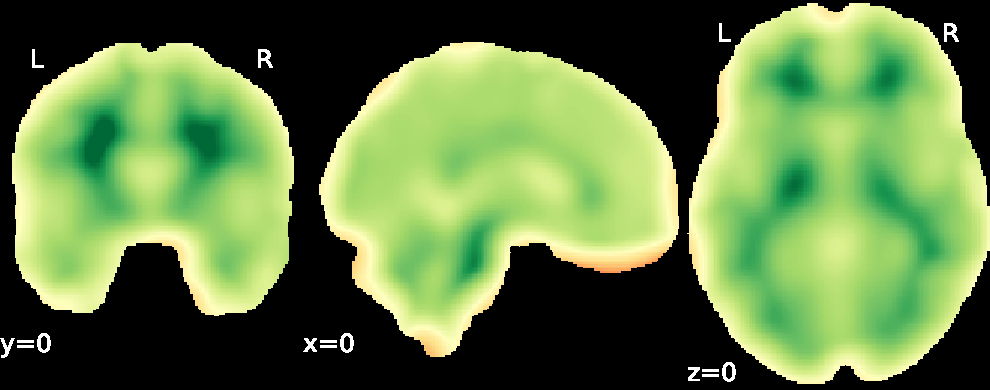
\includegraphics[width=\textwidth]{figures/sig/15mm/rr_ds000256_sub-CTS201_sig.pdf}
        \end{subfigure}
        \begin{subfigure}[t]{0.2\paperheight}
            \centering
            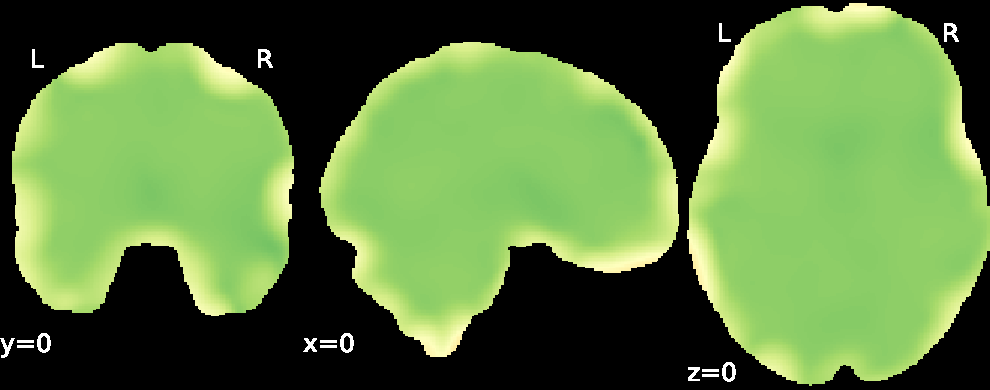
\includegraphics[width=\textwidth]{figures/sig/15mm/rs_ds000256_sub-CTS201_sig.pdf}
        \end{subfigure}
        \begin{subfigure}[t]{0.2\paperheight}
            \centering
            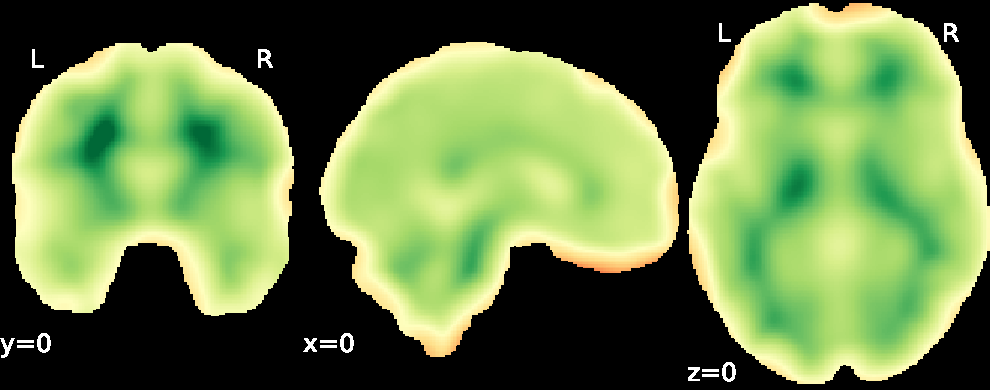
\includegraphics[width=\textwidth]{figures/sig/15mm/rr.rs_ds000256_sub-CTS201_sig.pdf}
        \end{subfigure} \\
        %% sub 4
        \begin{subfigure}[b][][c]{0.01\paperwidth} 4 \vspace*{15pt} \end{subfigure}
        \begin{subfigure}[t]{0.2\paperheight}
            \centering
            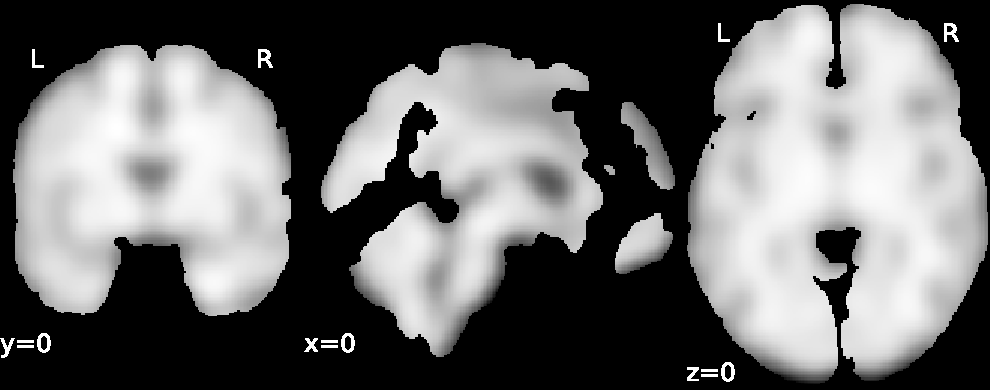
\includegraphics[width=\textwidth]{figures/sig/15mm/ieee_ds000256_sub-CTS210.pdf}
        \end{subfigure}
        \begin{subfigure}[t]{0.2\paperheight}
            \centering
            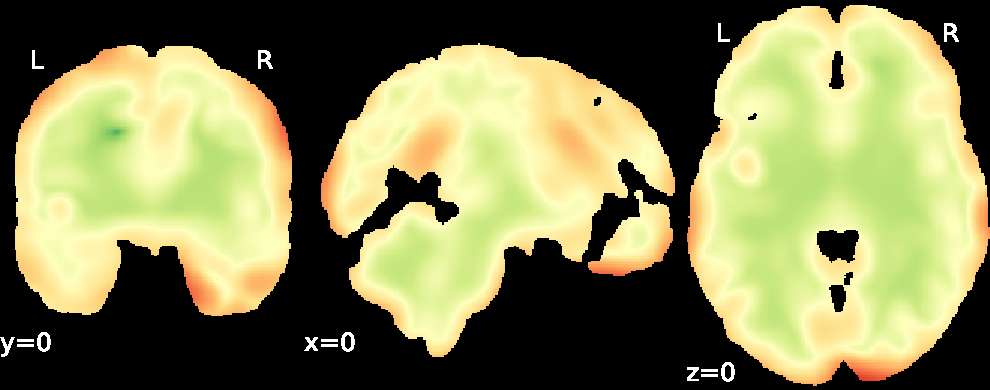
\includegraphics[width=\textwidth]{figures/sig/15mm/rr_ds000256_sub-CTS210_sig.pdf}
        \end{subfigure}
        \begin{subfigure}[t]{0.2\paperheight}
            \centering
            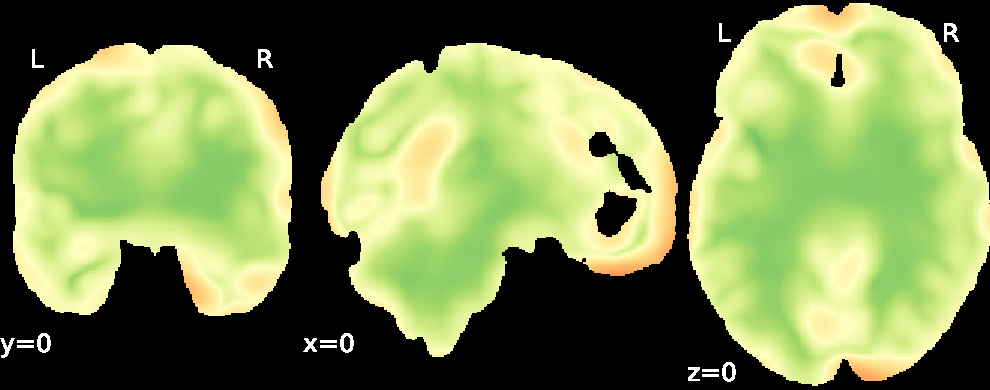
\includegraphics[width=\textwidth]{figures/sig/15mm/rs_ds000256_sub-CTS210_sig.pdf}
        \end{subfigure}
        \begin{subfigure}[t]{0.2\paperheight}
            \centering
            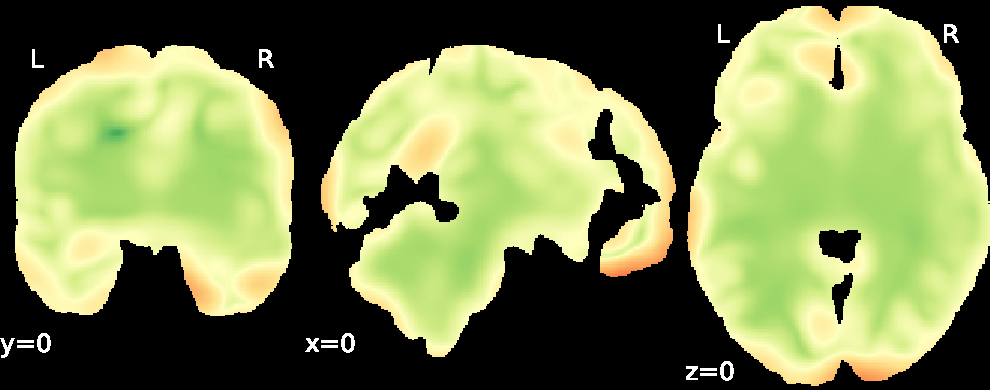
\includegraphics[width=\textwidth]{figures/sig/15mm/rr.rs_ds000256_sub-CTS210_sig.pdf}
        \end{subfigure} \\
        %% sub 5
        \begin{subfigure}[b][][c]{0.01\paperwidth} 5 \vspace*{15pt} \end{subfigure}
        \begin{subfigure}[t]{0.2\paperheight}
            \centering
            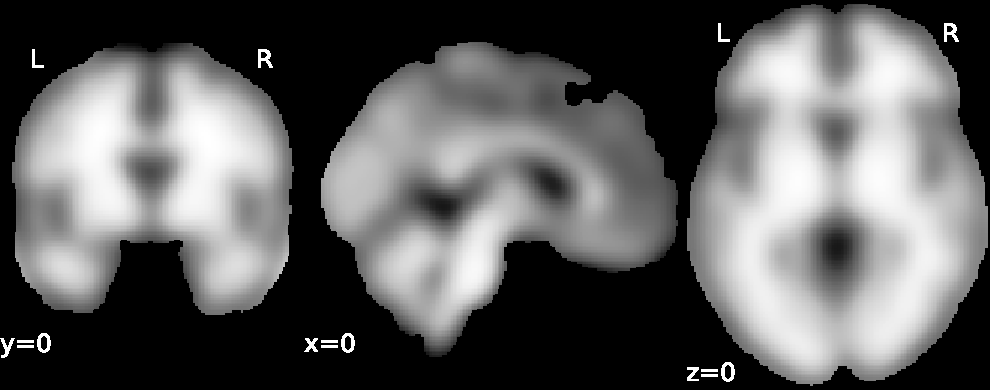
\includegraphics[width=\textwidth]{figures/sig/15mm/ieee_ds001748_sub-adult15.pdf}
        \end{subfigure}
        \begin{subfigure}[t]{0.2\paperheight}
            \centering
            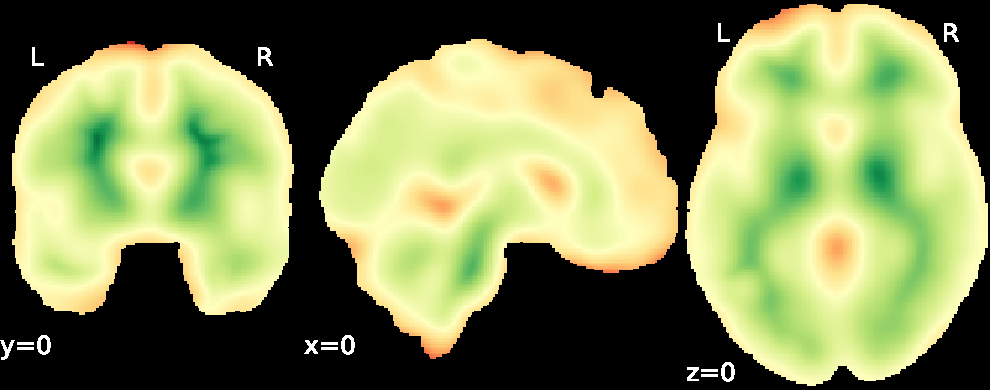
\includegraphics[width=\textwidth]{figures/sig/15mm/rr_ds001748_sub-adult15_sig.pdf}
        \end{subfigure}
        \begin{subfigure}[t]{0.2\paperheight}
            \centering
            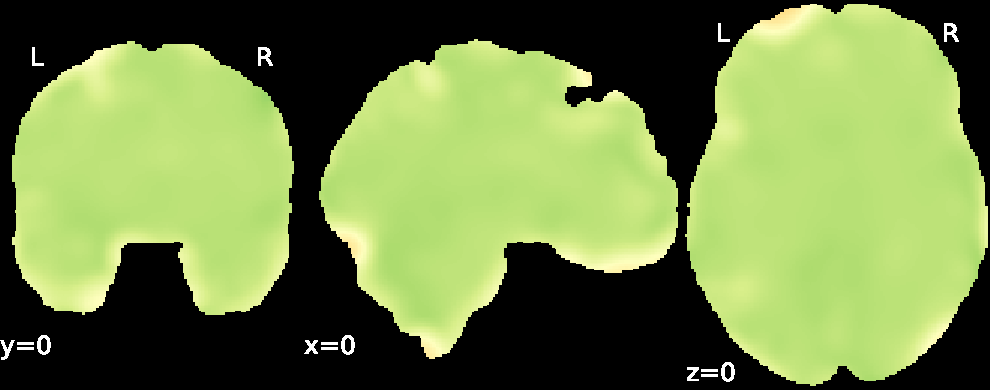
\includegraphics[width=\textwidth]{figures/sig/15mm/rs_ds001748_sub-adult15_sig.pdf}
        \end{subfigure}
        \begin{subfigure}[t]{0.2\paperheight}
            \centering
            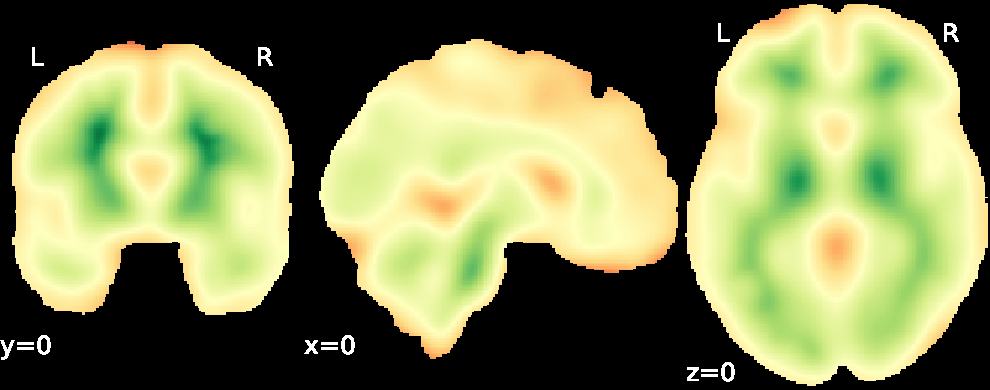
\includegraphics[width=\textwidth]{figures/sig/15mm/rr.rs_ds001748_sub-adult15_sig.pdf}
        \end{subfigure} \\
        %% sub 6
        \begin{subfigure}[b][][c]{0.01\paperwidth} 6 \vspace*{15pt} \end{subfigure}
        \begin{subfigure}[t]{0.2\paperheight}
            \centering
            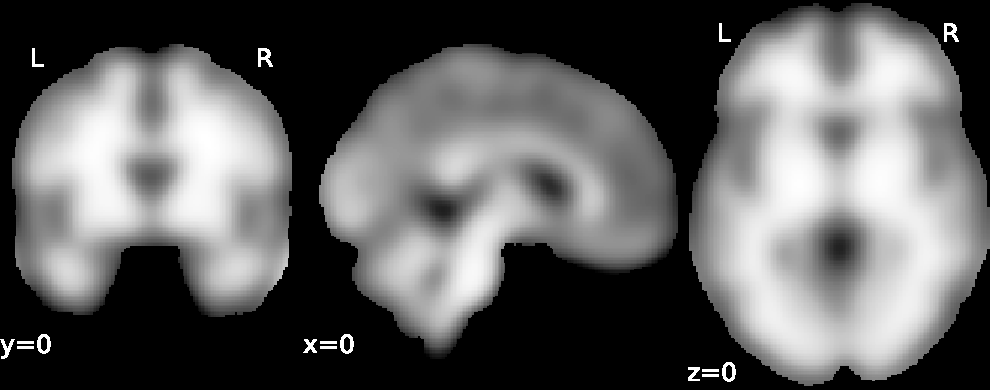
\includegraphics[width=\textwidth]{figures/sig/15mm/ieee_ds001748_sub-adult16.pdf}
        \end{subfigure}
        \begin{subfigure}[t]{0.2\paperheight}
            \centering
            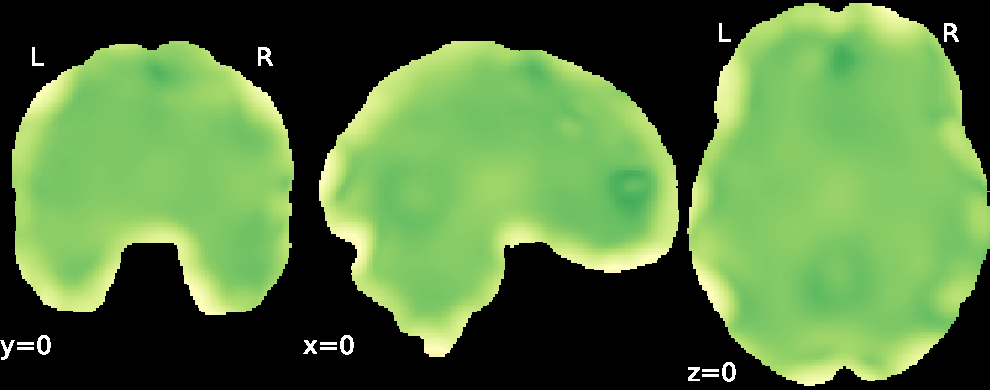
\includegraphics[width=\textwidth]{figures/sig/15mm/rr_ds001748_sub-adult16_sig.pdf}
        \end{subfigure}
        \begin{subfigure}[t]{0.2\paperheight}
            \centering
            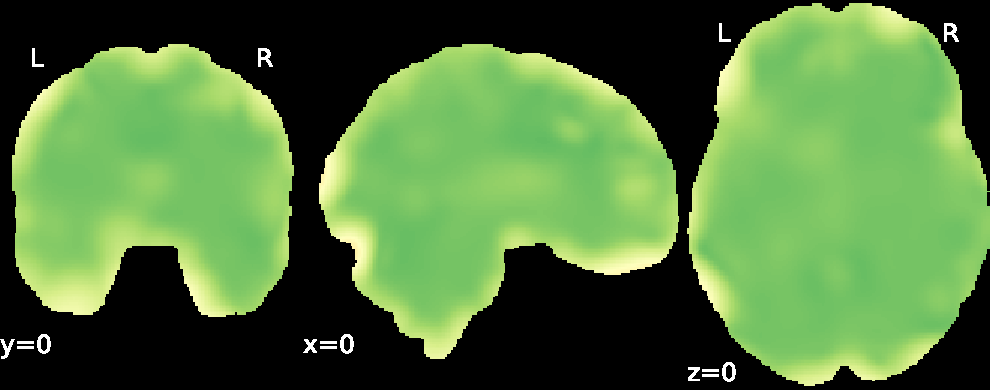
\includegraphics[width=\textwidth]{figures/sig/15mm/rs_ds001748_sub-adult16_sig.pdf}
        \end{subfigure}
        \begin{subfigure}[t]{0.2\paperheight}
            \centering
            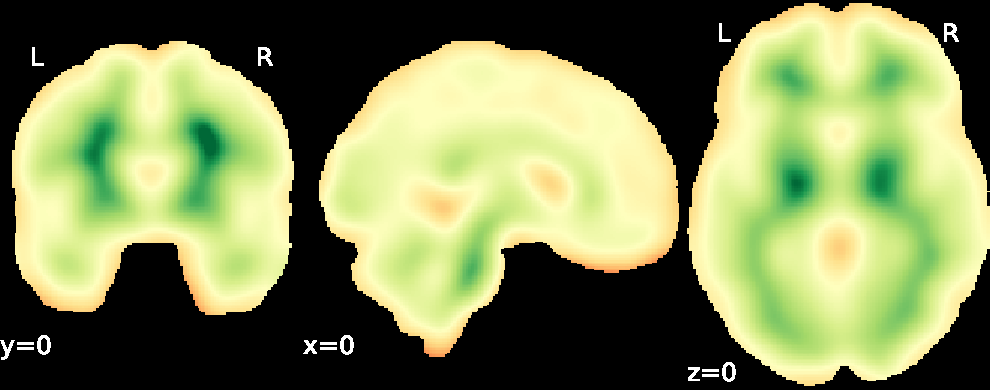
\includegraphics[width=\textwidth]{figures/sig/15mm/rr.rs_ds001748_sub-adult16_sig.pdf}
        \end{subfigure} \\
        %% sub 7
        \begin{subfigure}[b][][c]{0.01\paperwidth} 7 \vspace*{15pt} \end{subfigure}
        \begin{subfigure}[t]{0.2\paperheight}
            \centering
            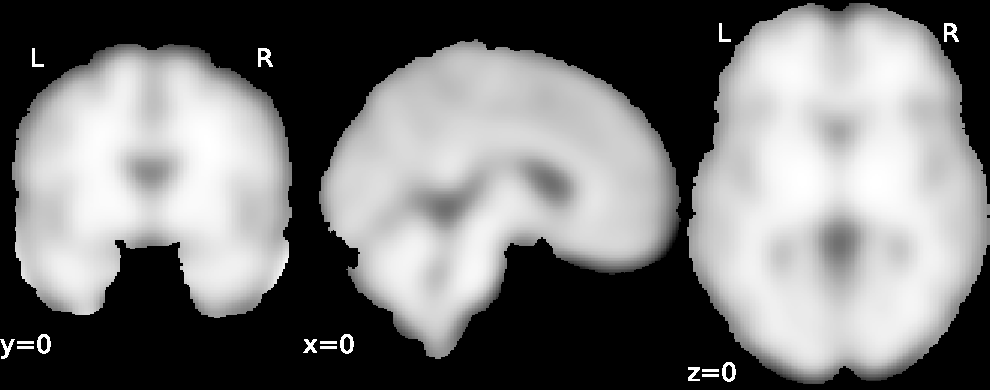
\includegraphics[width=\textwidth]{figures/sig/15mm/ieee_ds002338_sub-xp201.pdf}
        \end{subfigure}
        \begin{subfigure}[t]{0.2\paperheight}
            \centering
            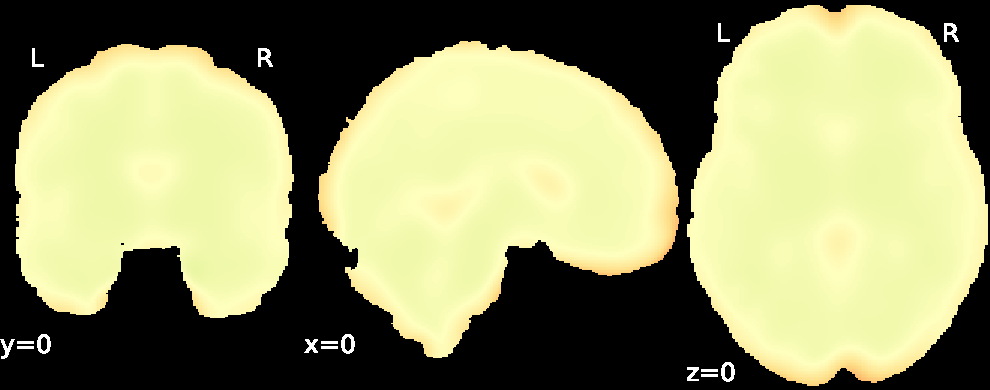
\includegraphics[width=\textwidth]{figures/sig/15mm/rr_ds002338_sub-xp201_sig.pdf}
        \end{subfigure}
        \begin{subfigure}[t]{0.2\paperheight}
            \centering
            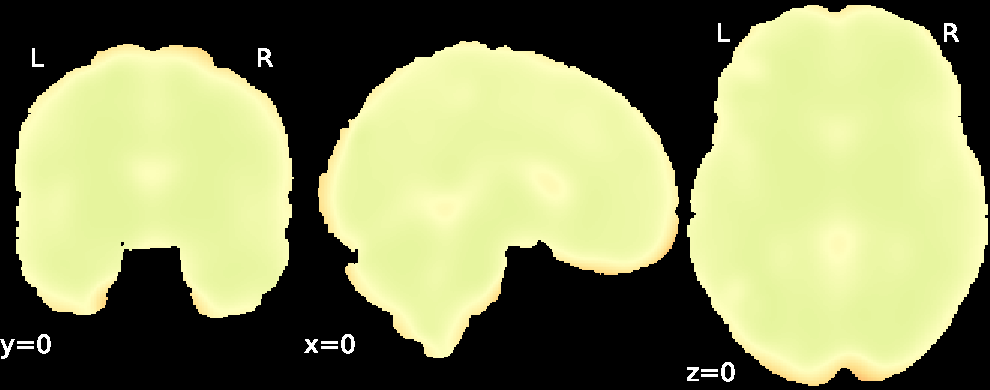
\includegraphics[width=\textwidth]{figures/sig/15mm/rs_ds002338_sub-xp201_sig.pdf}
        \end{subfigure}
        \begin{subfigure}[t]{0.2\paperheight}
            \centering
            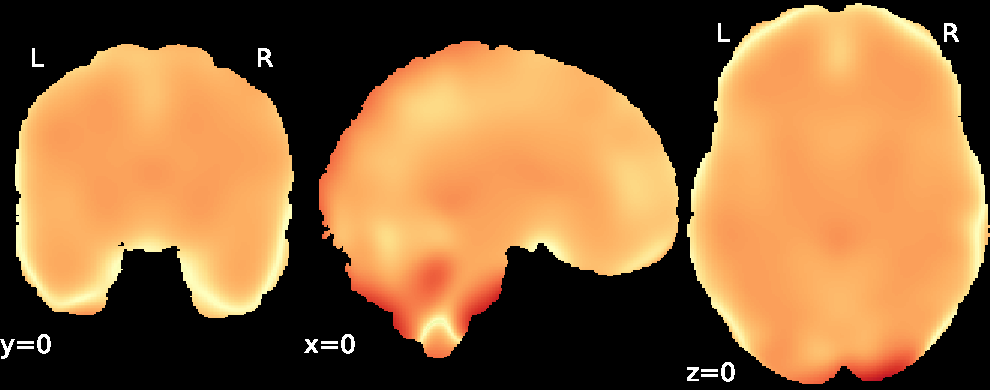
\includegraphics[width=\textwidth]{figures/sig/15mm/rr.rs_ds002338_sub-xp201_sig.pdf}
        \end{subfigure} \\
        %% sub 8
        \begin{subfigure}[b][][c]{0.01\paperwidth} 8 \vspace*{15pt} \end{subfigure}
        \begin{subfigure}[t]{0.2\paperheight}
            \centering
            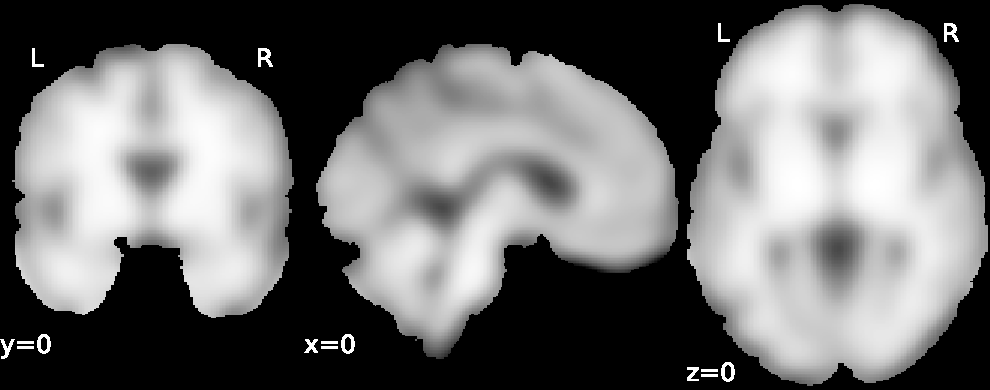
\includegraphics[width=\textwidth]{figures/sig/15mm/ieee_ds002338_sub-xp207.pdf}
        \end{subfigure}
        \begin{subfigure}[t]{0.2\paperheight}
            \centering
            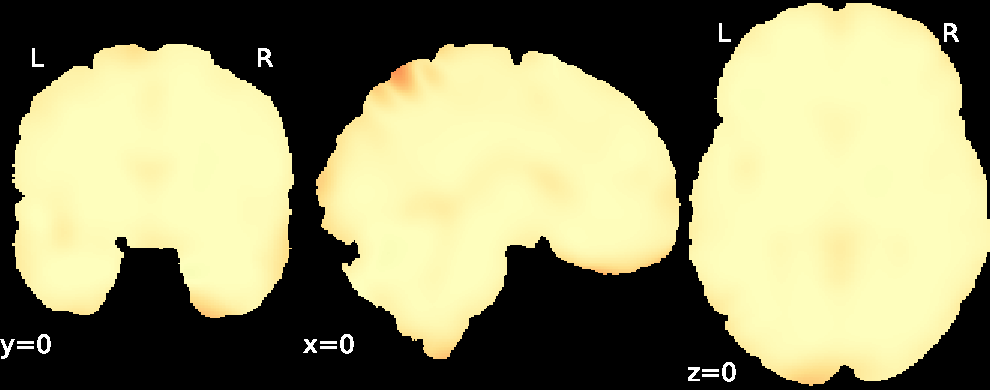
\includegraphics[width=\textwidth]{figures/sig/15mm/rr_ds002338_sub-xp207_sig.pdf}
        \end{subfigure}
        \begin{subfigure}[t]{0.2\paperheight}
            \centering
            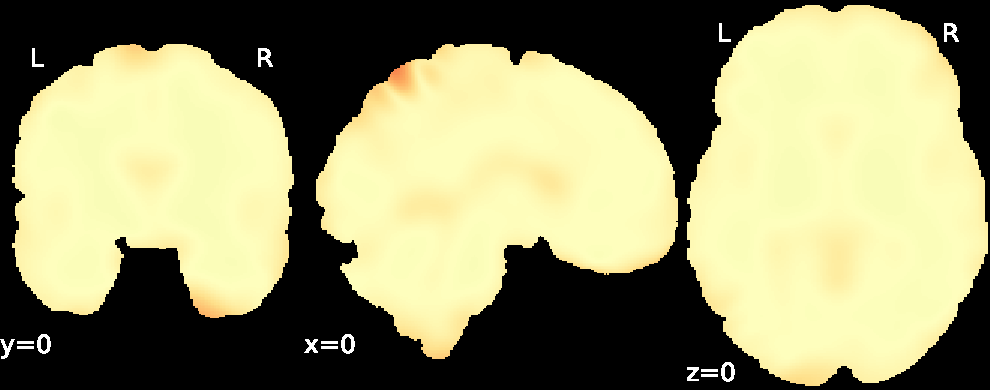
\includegraphics[width=\textwidth]{figures/sig/15mm/rs_ds002338_sub-xp207_sig.pdf}
        \end{subfigure}
        \begin{subfigure}[t]{0.2\paperheight}
            \centering
            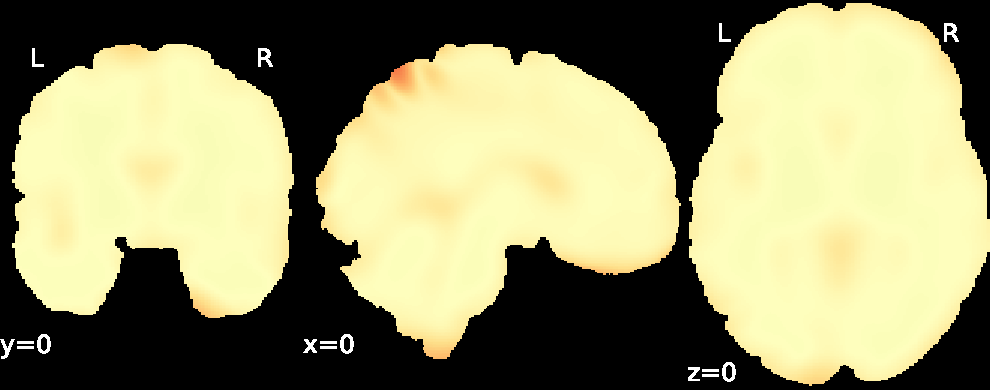
\includegraphics[width=\textwidth]{figures/sig/15mm/rr.rs_ds002338_sub-xp207_sig.pdf}
        \end{subfigure} \\
        \hspace*{6cm} 0 \tikz[baseline=(current bounding box.south)]{
            \draw[left color=red, right color=green!50!black, middle color=yellow]
            (0,0) rectangle (8,0.3);} 12 bits
        \caption{Uncertainty measured for subjects 1 to 8 (from top to bottom) across n=30 for
            (from right to left) IEEE, RR, RS and RR+RS perturbed samples with a spatial smoothing applied (FWHM=15mm). }
        \label{fig:uncertainty-maps}

    \end{figure}
\end{landscape}


\subsection{Non-regression test evaluations}

\paragraph{Leave-one-out evaluation.} We implemented a ``leave-one-out" (LOO)
evaluation by constructing the non-regression test $n$ times for $n-1$ perturbed results
and applying it to the remaining perturbed result. We model the LOO test
using a binomial variable $B(n,1-\alpha)$
where $n$ is the number of repetitions and $1-\alpha$ is
the probability of success of a repetition. Under $H_0$ for all voxels, we
expect the following
bound to be verified:
\[
    1-F(\mathds{1}_n;n,1-\alpha) \leq \alpha_0
\]
where $F(x;n,p)$ is the cumulative distribution function of the Binomial law $B(n,p)$, and
$\alpha_0=0.05$.

We applied leave-one-out validation for
different  confidence values (1-$\alpha$) and different FWHM  values for the
3 types of perturbations (Figure~\ref{fig:loo_bonferroni}). As expected, tests
become increasingly permissive for increasing values of $\alpha$ (reduced
confidence) and increasing values of FWHM. As previously observed, the 3 perturbation types
behave similarly. For each subject, $\alpha$ and FWHM values exist such that
the LOO test passes. However, these values importantly vary across subjects, presumably
due to heterogeneous data quality. To pass the LOO
test with $\alpha=0.05$ for RR perturbations,
subjects 2, 6, 7 and 8 require a smoothing size of FWHM=12mm and
subjects 3, 5 require FWHM=15mm. Subjects 1 and 4 never pass the LOO test
at this confidence level.

% For each type of perturbation, we
% define "best operating values" $\alpha^\star$ and $\fwhm^\star$ for these parameters
% such that:
% \begin{equation}
%     (\alpha^\star, \fwhm^\star) = \min\left(\underset{(\alpha, \fwhm)}{\mathrm{argmax}}\left( S(\alpha,\fwhm)\right)\right),
% \end{equation}
% where $S(\alpha, \fwhm)$ is the number of subjects that pass the test for
% $\alpha$ and $\fwhm$ and the minimum is determined using the lexicographic
% order on $A \times F$ where $A$ is the set of all $\alpha$ values and $F$ is the
% set of all FWHM values. $\alpha^\star$ is the minimum value of $\alpha$ for which
% the maximal number of subjects pass the test, and $\fwhm^\star$ is the minimal
% smoothing kernel size such that the maximal number of subjects pass the test
% with $\alpha^\star$. \TG{comment on $\alpha^\star$ and $\fwhm^\star$ values.}

% It can be
% noted that among the 8 tested subjects, subject 210 never passes the test for RR
% or RS perturbations, and only passed the test for $\alpha^\star=0.2$ and
% $\fwhm^\star=20mm$ for the RR+RS perturbation. This is due to the fact that for
% many voxels in this subject's image, the confidence interval resulting from a
% Gaussian fit of the intensity distribution across perturbed samples does not
% properly reflect the distribution. A visual inspection of the image did not
% show any particular image artifact (e.g., motion) or atypical anatomical feature
% (e.g., unusually large ventricles) that could explain such variations. Finally,
% as detailed in Appendix~\ref{appendix:multiple-comparison-tests}, the other
% tested methods for multiple comparison corrections led to similar conclusions.



\begin{figure}
    \centering
    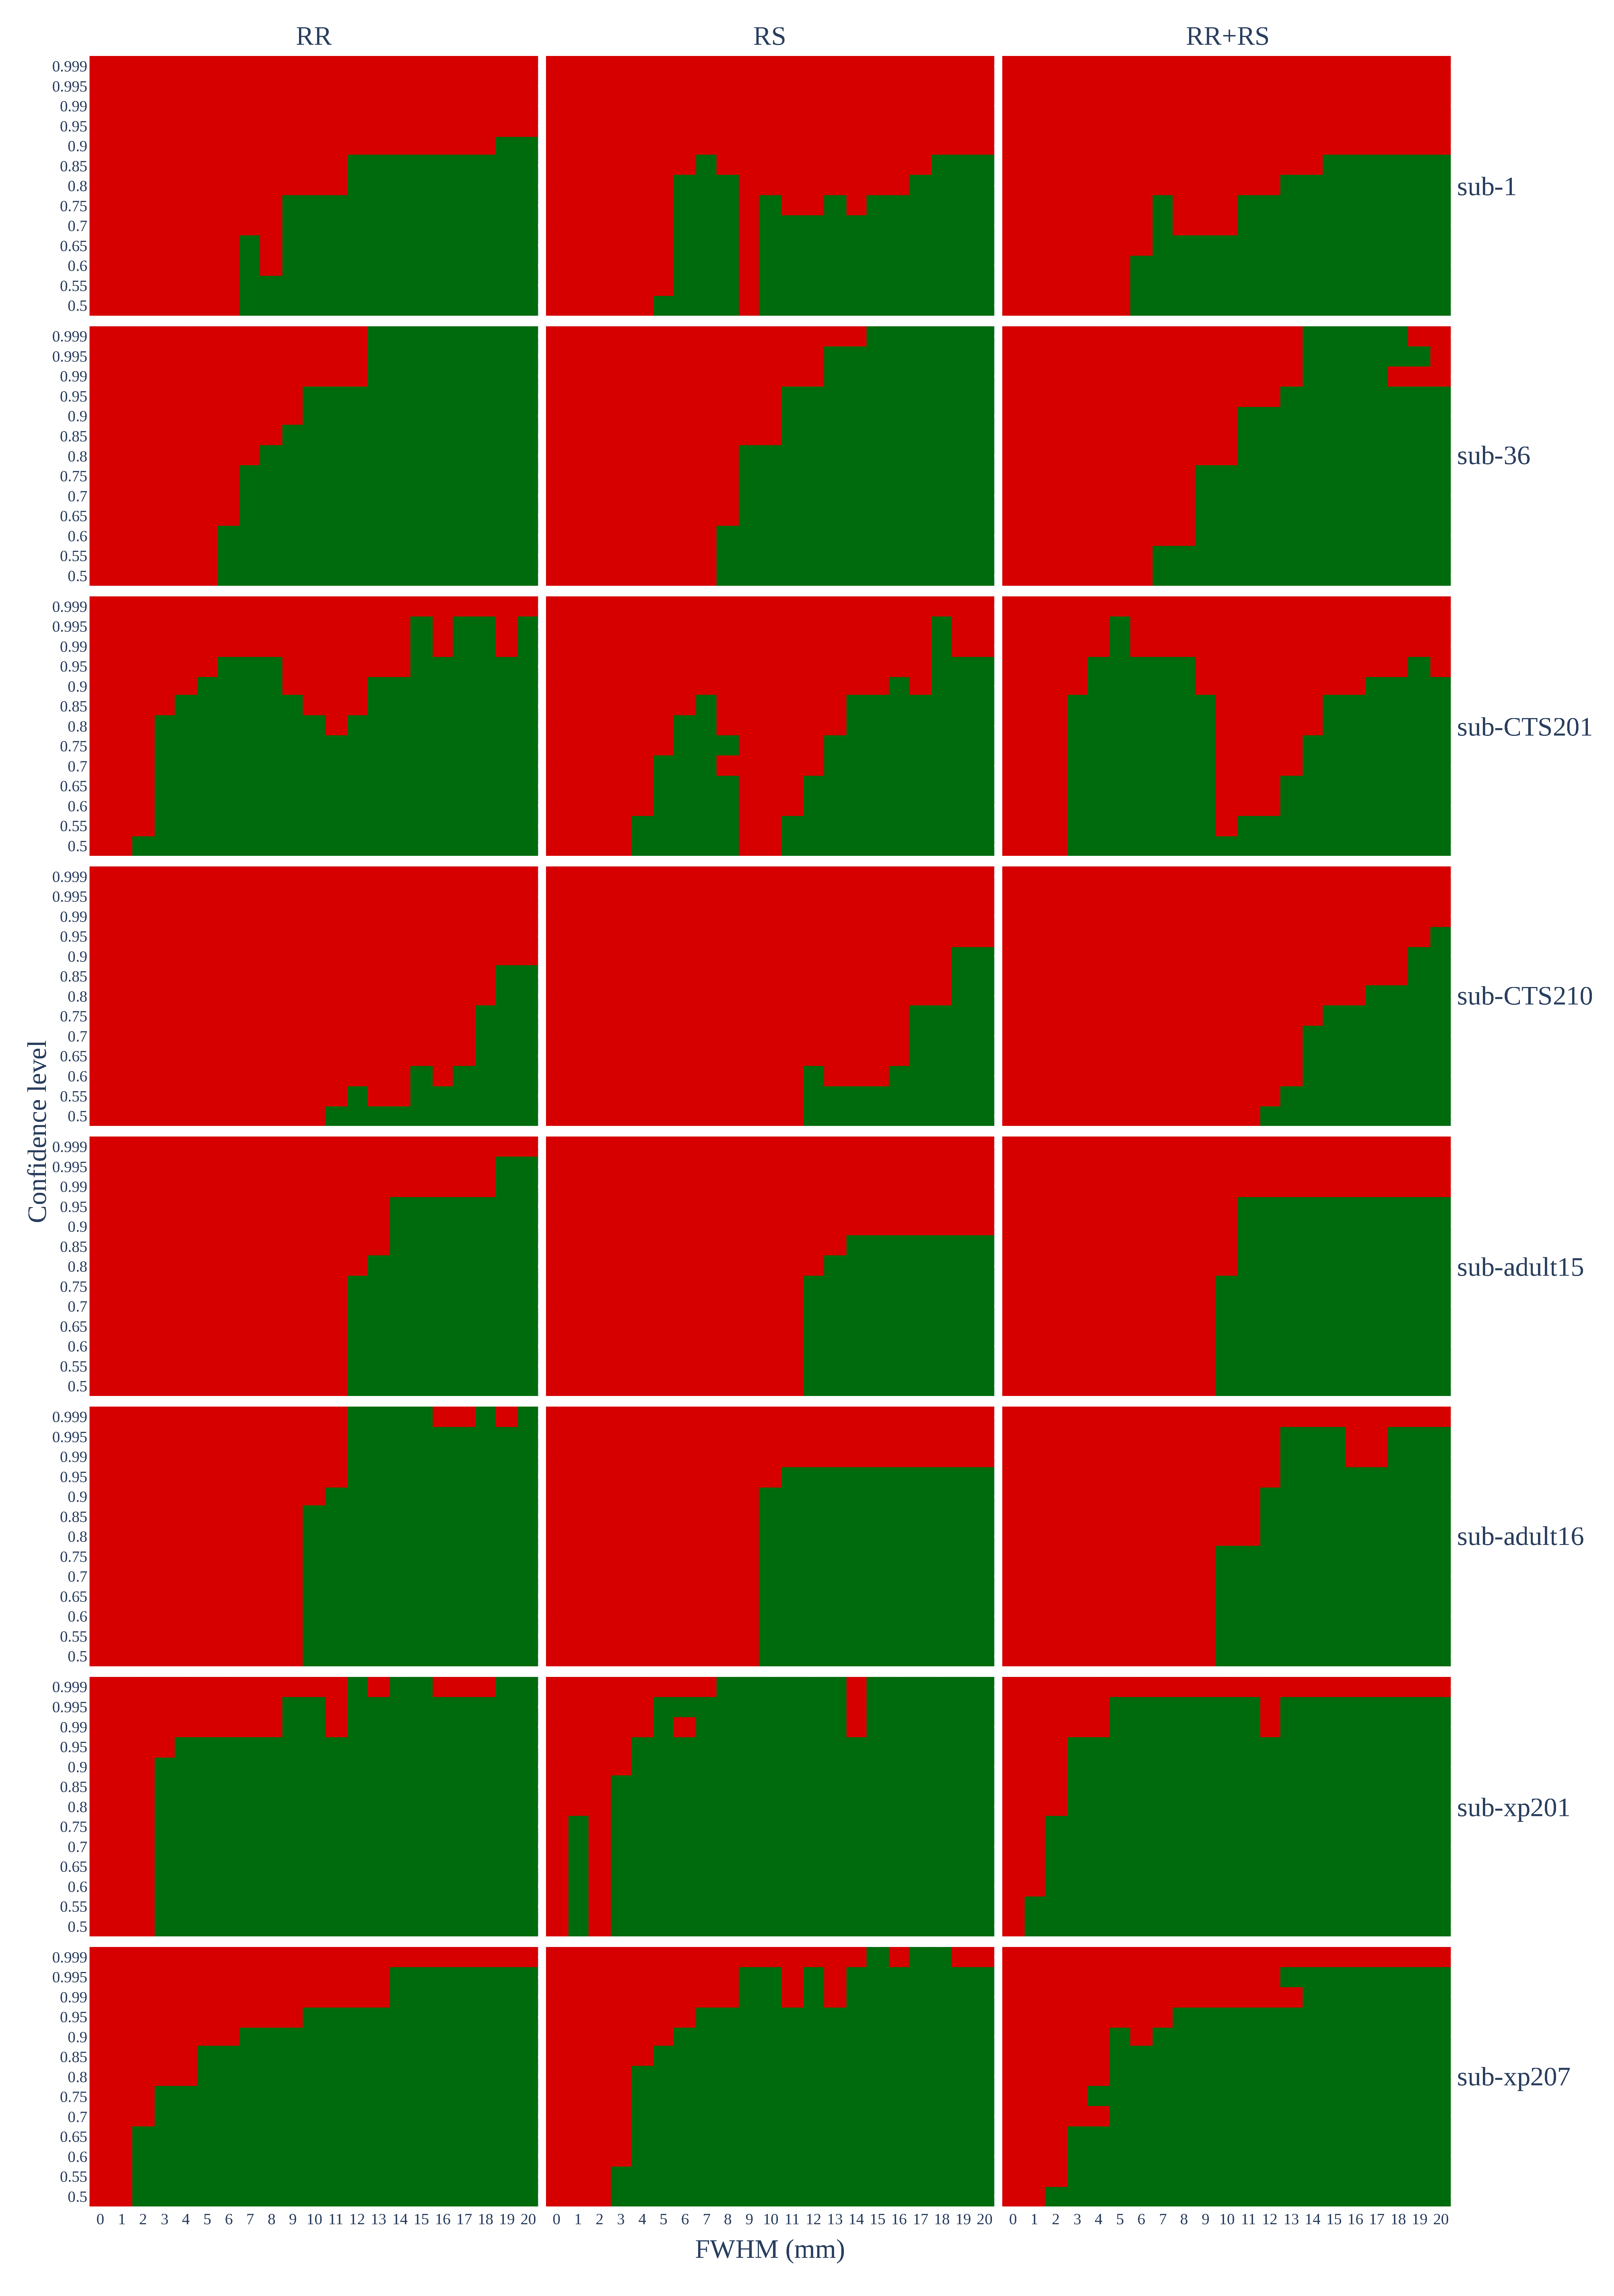
\includegraphics[width=\linewidth]{figures/exclude_mct_fwe_bonferroni.pdf}
    \caption{Leave-one-out evaluation for non-regression tests.
        Binomial one-tailed test with a confidence level at 95\%.
        Red: failed the test. Green: passed the test.}
    \label{fig:loo_bonferroni}
\end{figure}


\paragraph{IEEE check.} We check that the IEEE results (computed without random
perturbations) are correclty captured by our non-regression test. The IEEE check
constructs the non-regression test from the $n$ perturbed results and applies it
to each of the 8 IEEE results (one per subject). The purpose of this test is
twofolds: (1) be able to capture the IEEE results considered as part of the
reference distribution and (2) be able to correclty reject an observation not
comming from the reference distribution (here from an other subject).

Figure~\ref{fig:ieee-check} shows the result for increasing values of $\alpha$
and FWHM for the 3 types of perturbations. Each cell is a comparison matrix
with the subject used as reference on the row and the subject used as target on
the colum, following the subject indexing in Table~\ref{table:dataset_info}. The
transparent black line highlights the diagonal corresponding to the tests using
the same subject for the reference and the target. We expect the cell to have
green values on its diagonal and red values outside.

We first observe that none of the inter-subject tests fail which means that our
test is sufficiently specific to detect the inter-subject variability even with
high smoothing kernel size. However, the test lacks sensitivity for low FWHM
sizes, suggesting that the learning sample is too small. But most importantly,
it exists a $\alpha$ and FWHM pair for each subject such that the IEEE check
passes. Hence, the IEEE check passes with FWHM=15mm for all subjects and
$\alpha$ values in RR pertubations.

\begin{figure}
    \centering
    \begin{subfigure}[t]{0.7\linewidth}
        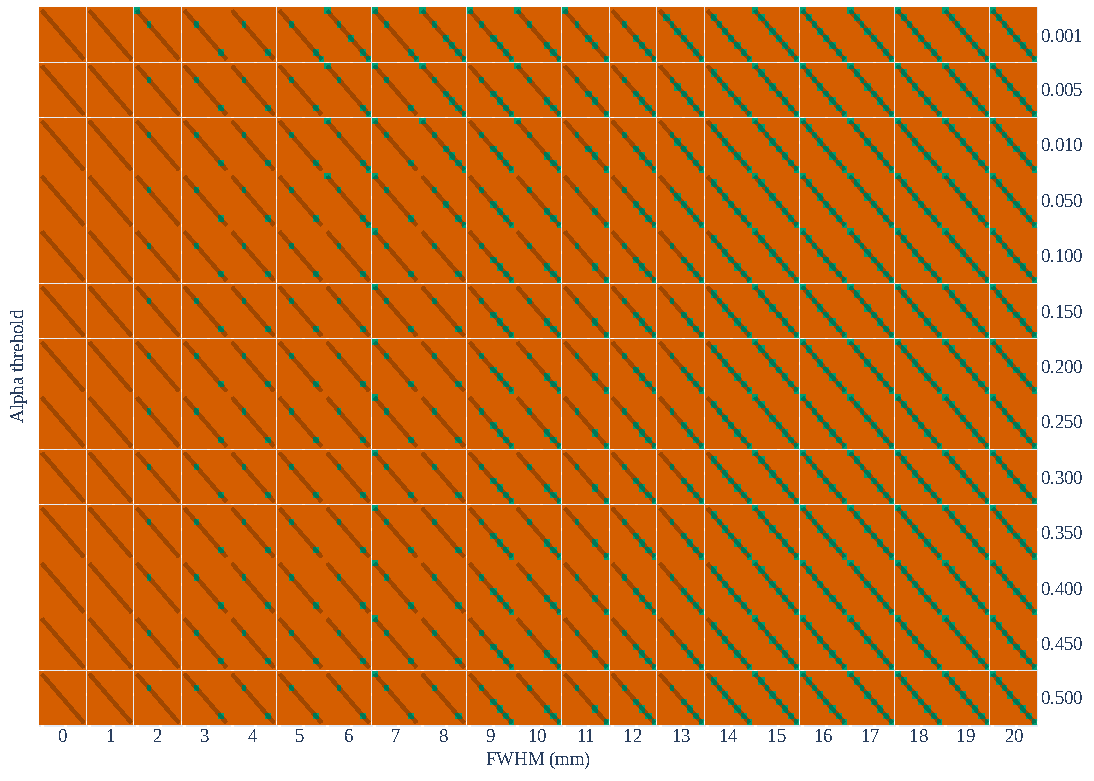
\includegraphics[width=\linewidth]{figures/inter-subject/one_mct_fwe_bonferroni_RR.pdf}
    \end{subfigure}
    \begin{subfigure}[t]{0.7\linewidth}
        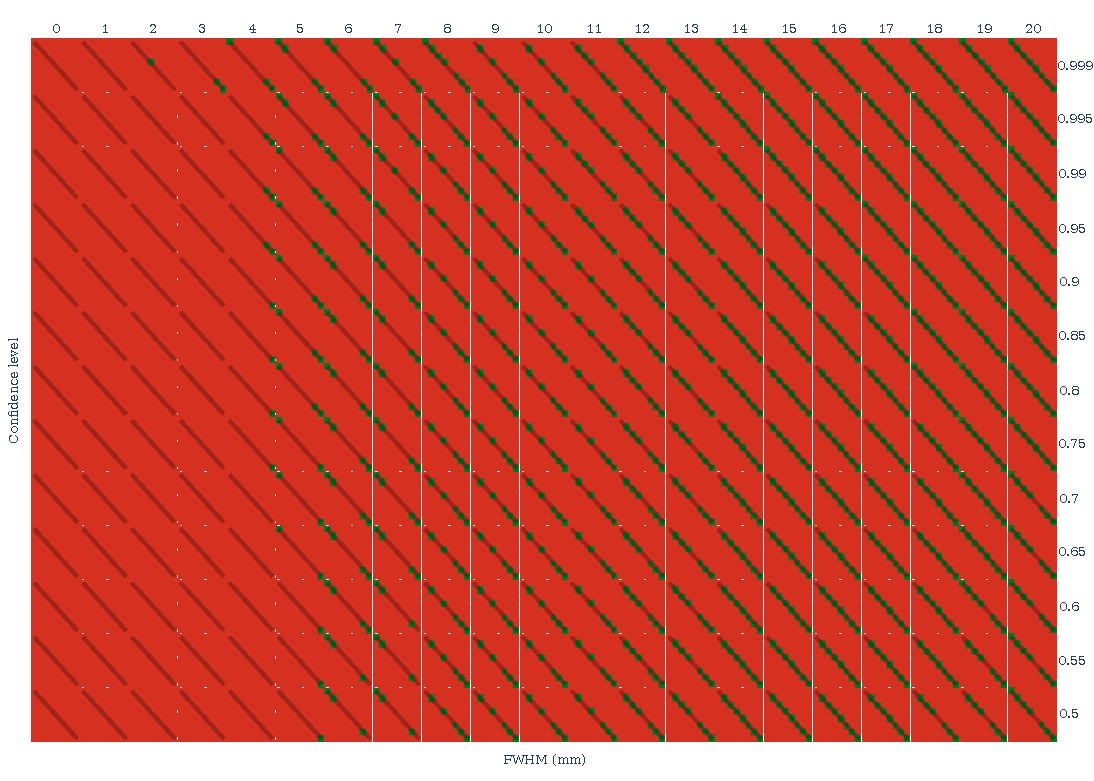
\includegraphics[width=\linewidth]{figures/inter-subject/one_mct_fwe_bonferroni_RS.pdf}
    \end{subfigure}
    \begin{subfigure}[t]{0.7\linewidth}
        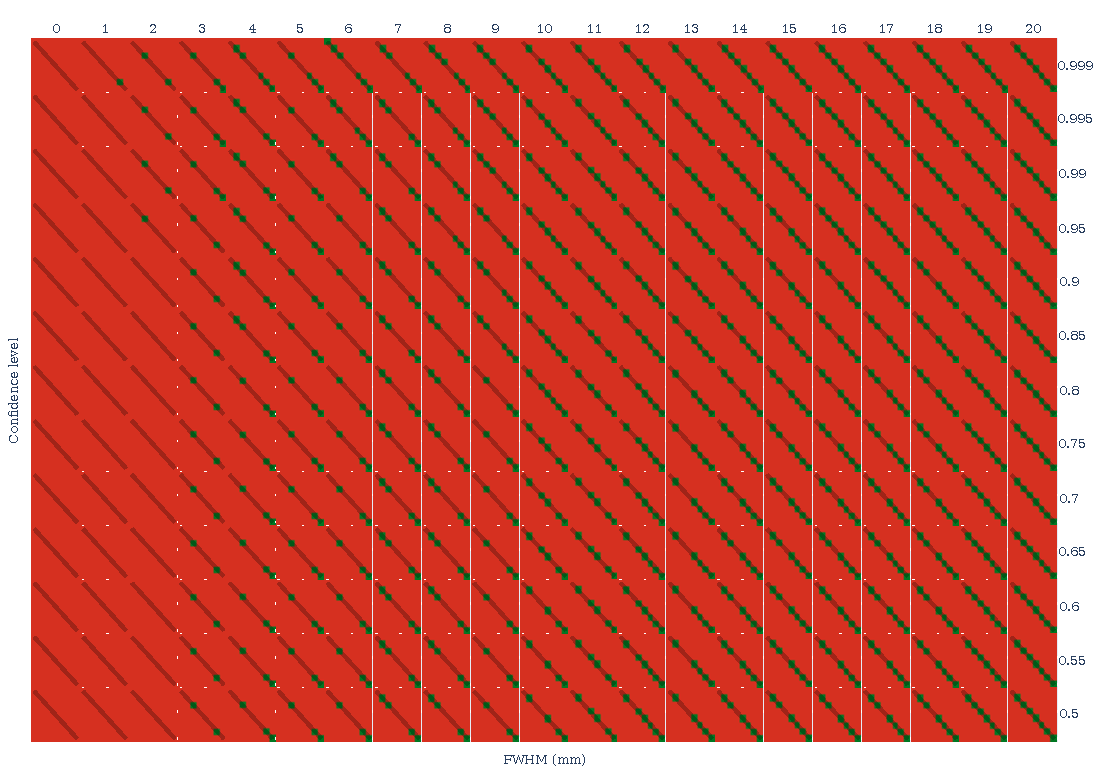
\includegraphics[width=\linewidth]{figures/inter-subject/one_mct_fwe_bonferroni_RR-RS.pdf}
    \end{subfigure}
    \caption{Inter-subject check for from top to bottom RR, RS and RR+RS modes (bonferroni)}
    \label{fig:ieee-check}
\end{figure}

\paragraph{Corrupted template check.}

\begin{figure}
    \centering
    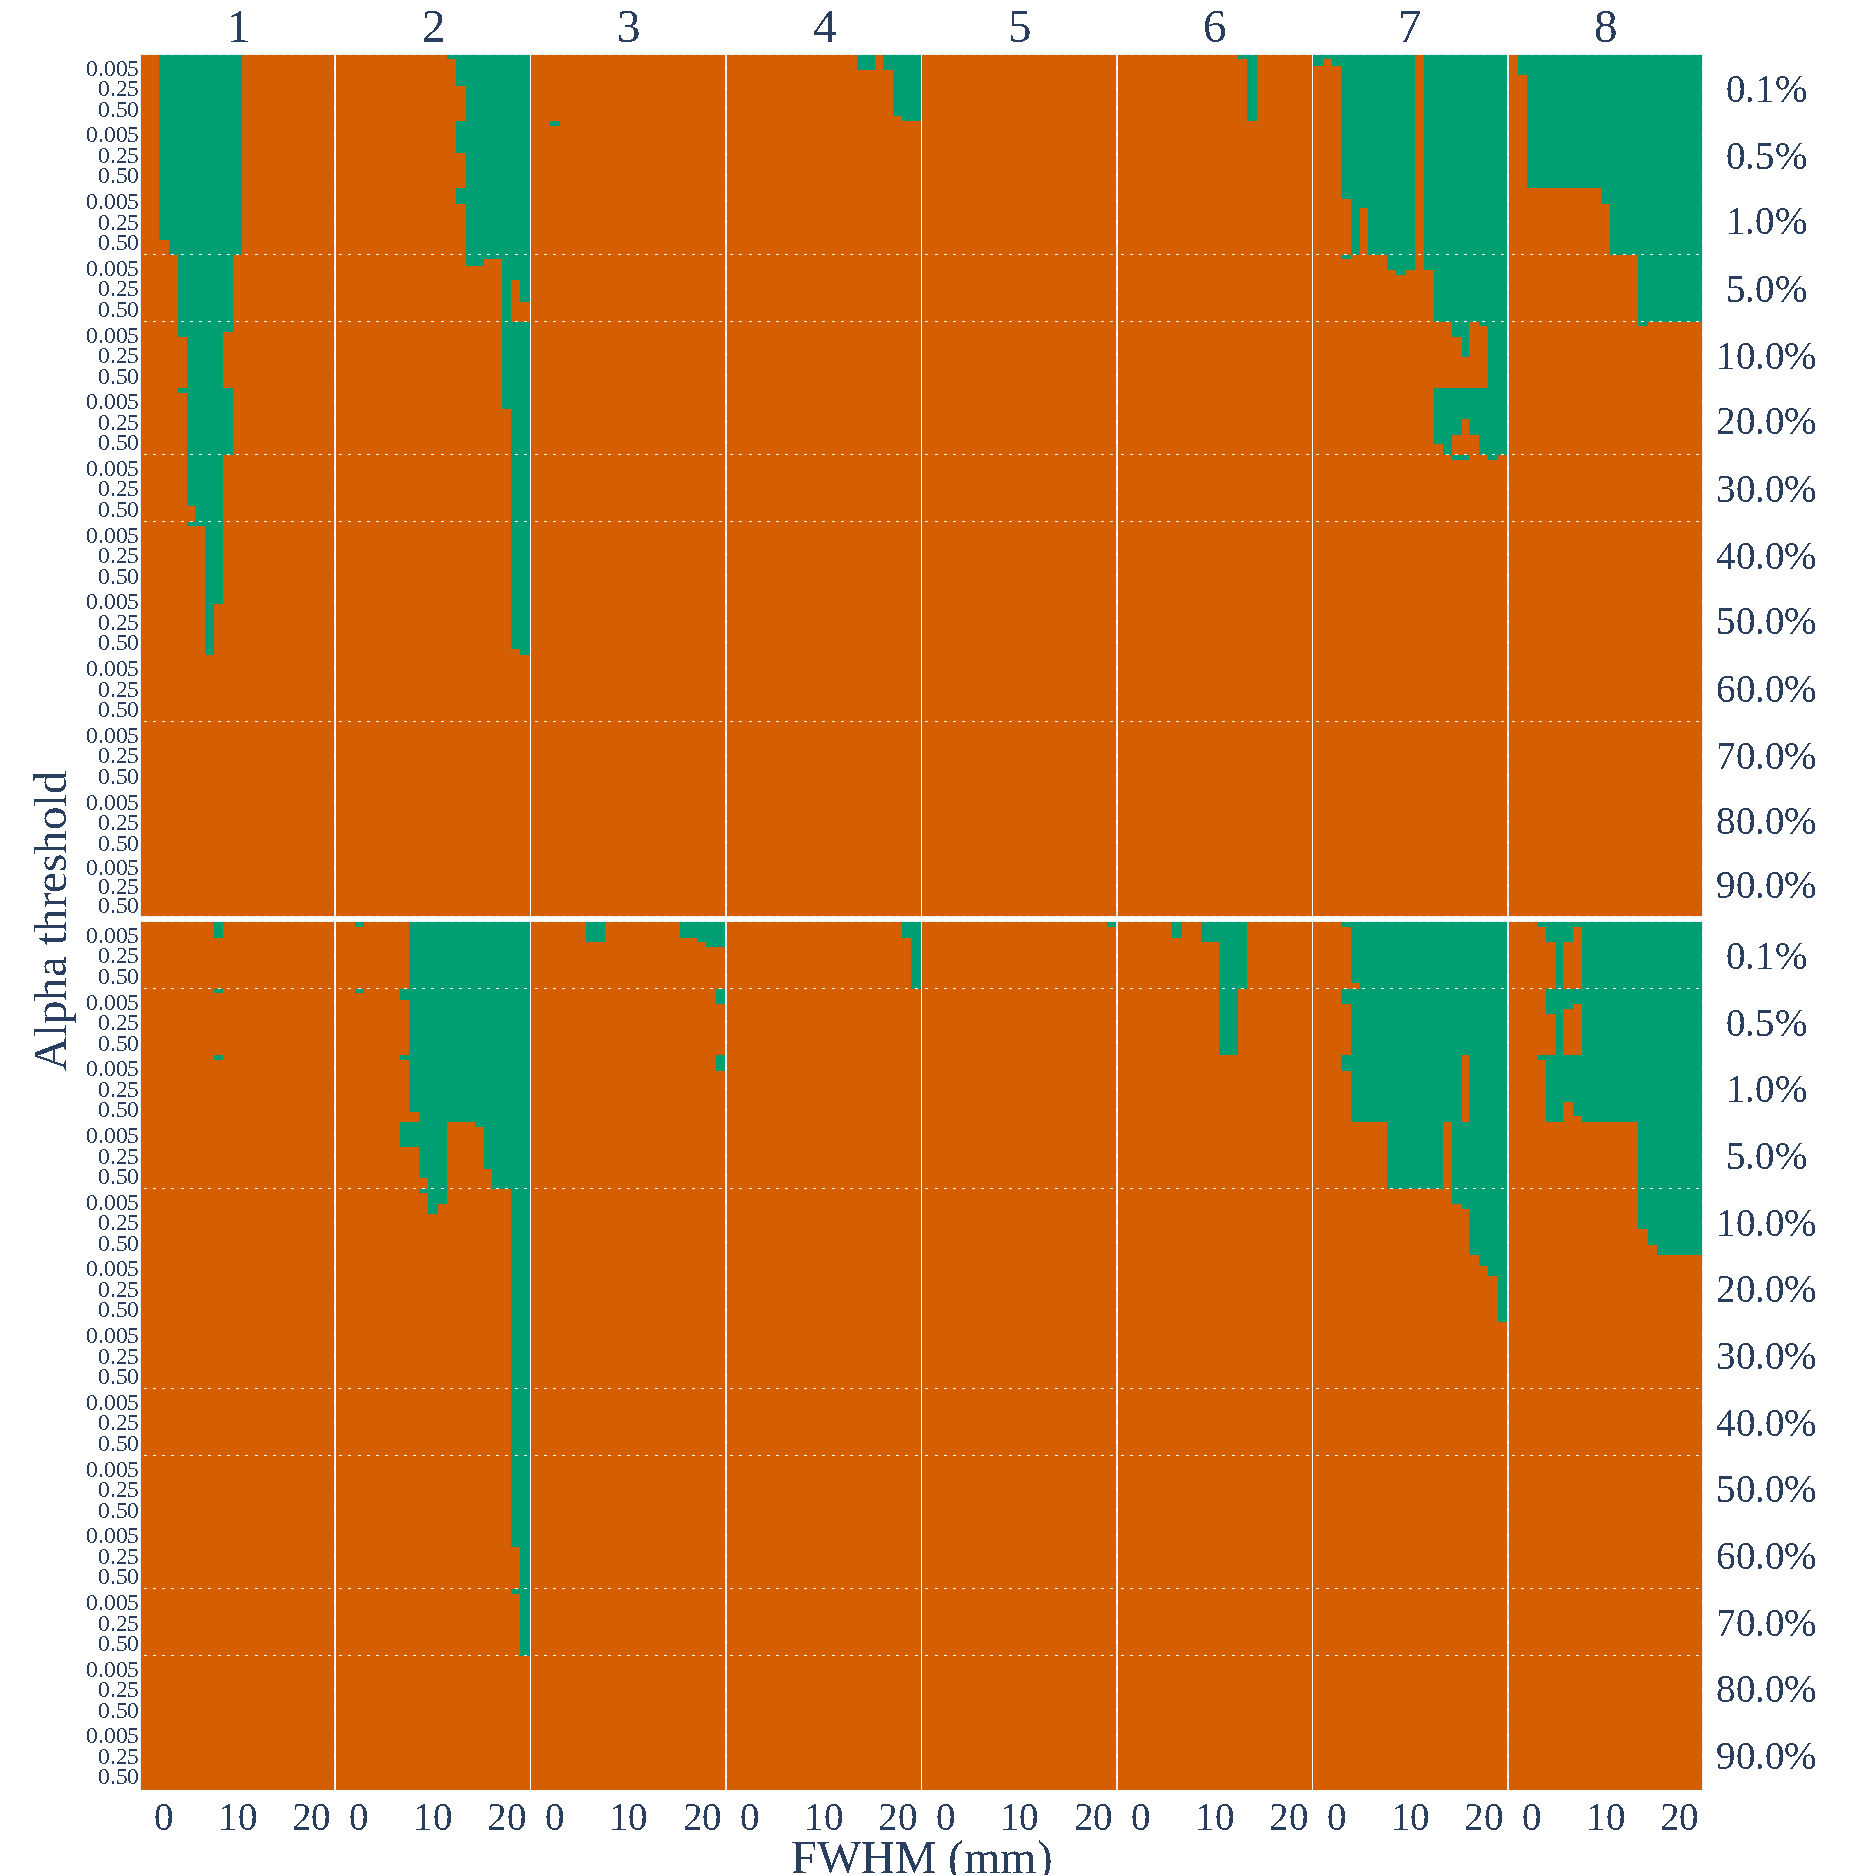
\includegraphics[width=\linewidth]{figures/template/template_fwe_bonferroni.pdf}
    \caption{Corrupted template check for RR, RS and RR+RS mode (bonferroni)}
    \label{fig:template_bonferroni}
\end{figure}

Image registration is a fundamental step during the pre-preprocessing to enable
statistical analyses. This step consists on realigning an input image (user
space) to a common space (template space). To do so, it exists several templates
representing a normal structural brain and \fmriprep uses the
MNI152NLin2009cAsym template from ... (REF) by default. The quality of the template will
condition the quality of the registred image. Hence, errors in the template
should lead to substential differences in the registred images. We use this
principle to build this check and to determine that our non-regression correctly
captures these variabilities induced.

To do so, we generated 13 noised versions of the MNI152NLin2009cAsym template
where we simulate "dead voxels" by setting the voxels intensity to 0 for a
fraction of the intracranial voxels. Each voxels had the same probability to be
drawn no matter its localization or tissue type in the brain. We then executed
\fmriprep in IEEE mode (without random perturbations) for each "corrupted
template" on each subjects.

Figures~\ref{fig:template_bonferroni} shows the results for increasing values of
$\alpha$ and FWHM for the 3 types of pertubations. On the left is the percentage
of "dead voxels" introduced inside the masked brain. First, the sensitivity of
the test to the "dead voxels" in not the same following the subjects. On one
hand, the test rejects the subjects 1, 2, 5 and 6 for small percentages of noise
($\leq 1\%$) even for high FMWH levels. On the other hand, subjects 3, 4, 7 and
8 require a high percentage of noise (80\% for highest level of smoothing) to be
rejected by the test. This distinction between the two groups of subjects is
correlated to the average number of significant bits
(Figure~\ref{fig:significant-digits}), the first group being the one with the
highest average number of significant bits. This distinction is also clearly
visible when we look at the uncertainty maps at FMWH=5mm
(Figure~\ref{fig:uncertainty_5mm}). This correlation may mean that
the test is more permissive to high percentage of "dead voxels" for
subject having the highest uncertainty (or lowest number of significant bits).

\subsection{Non-regression test application to environment updates}

In this section, we explore the result of the non-regression test in different
environements. The goal is to detect factors causing results to outside accepted
variability bounds. We executed \fmriprep in IEEE mode by varying two factors:
the CPU architecture to execute on and the \fmriprep version.

\paragraph*{Architecture.} Figure~\ref{fig:arch_bonferroni} shows the results of
the non-regression test with the Bonferroni correction for increasing $\alpha$
and FWHM values for the 3 types of perturbations. Table~\ref{tab:index-arch-map}
gives the mapping between the architecture used and the letter present on the
left y-axis. We see that the architecture used has no impact on the
non-regression test since results are identical accross architecture for a
subject and a perturbation mode given. For subject 1, we see that the
variability of the non-regression test results is more important. In conclusion,
the perturbation mode used to build the test is more important than the
architecture used.


\begin{figure}
    \centering
    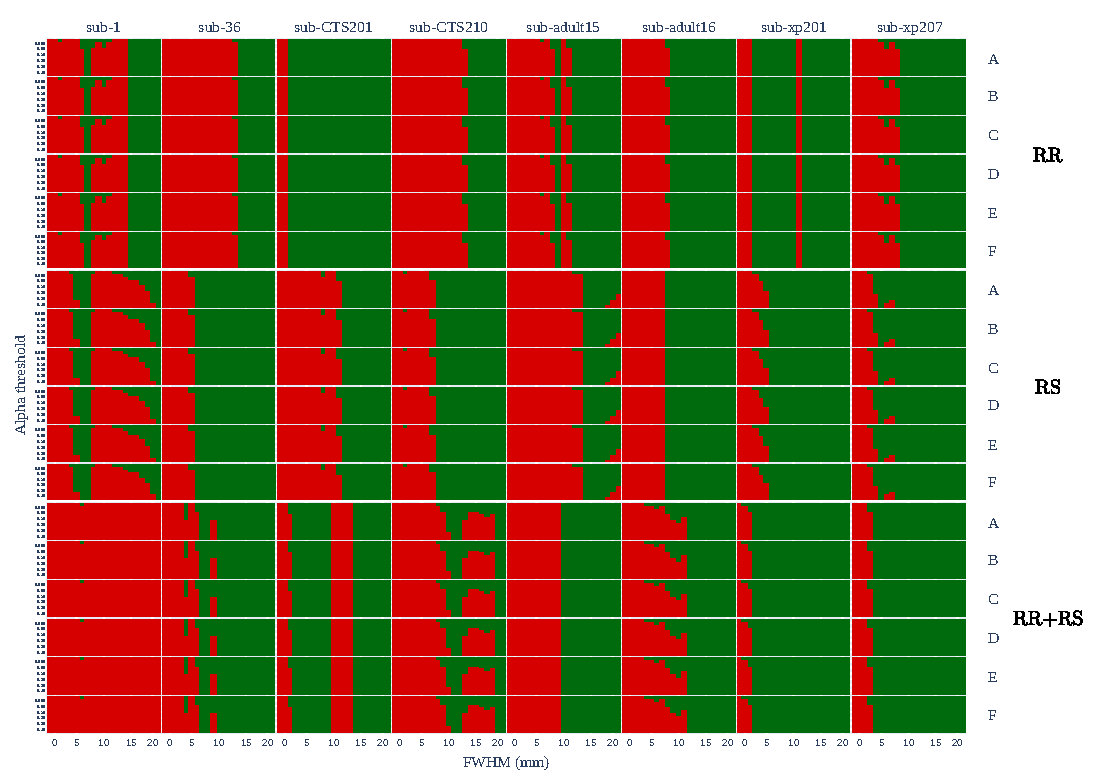
\includegraphics[width=\linewidth]{figures/arch/arch_mct_fwe_bonferroni_.pdf}
    \caption{Bonferroni corrected test application on different CPU architectures}
    \label{fig:arch_bonferroni}
\end{figure}

\begin{table}
    \begin{center}
        \begin{tabular}{c|l}
            Index & Architecture                   \\
            \hline
            A     & AMD Rome 7532                  \\
            B     & Intel E5-2683 v4 Broadwell     \\
            C     & Intel Silver 4216 Cascade Lake \\
            D     & Intel Platinum 8160F Skylake   \\
            E     & Intel Gold 5120 Skylake        \\
            F     & Intel Gold 6238 Cascade Lake
        \end{tabular}
    \end{center}
    \caption{Index of CPU architectures for Figure~\ref{fig:arch_bonferroni}. We use architecture A as reference.}
    \label{tab:index-arch-map}
\end{table}

\paragraph*{\fmriprep versions.} Figure~\ref{fig:version_bonferroni} shows the results of the non-regression test
with the Bonferroni correction for increasing $\alpha$ and FWHM values for the 3 types of perturbations.
On the left y-axis is the number of \fmriprep version used to compute the target image.
Overall, we see two oberserved two groups delimited by the version \texttt{20.2.5}.
From version \texttt{20.2.0} to \texttt{20.2.4}, results are identical for a given subject and perturbation mode.
Subject 4 passes for some confidence level and FWHM configurations. For the other major versions (21, 22 and 23)
the test reject all the subjects. This result suggests that code modifications introduced with version \texttt{20.2.5}
have modified the nature of the results produced by \fmriprep.
\TODO{find modifications and why it can explain the results}.

\begin{figure}
    \centering
    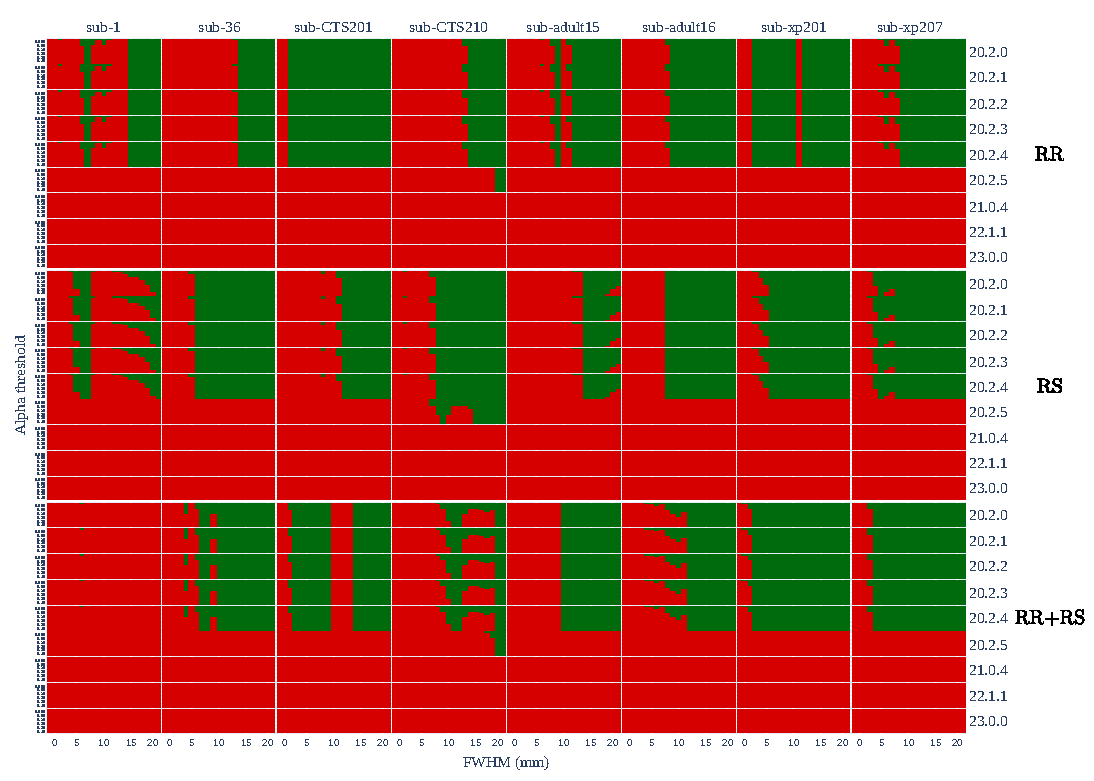
\includegraphics[width=\linewidth]{figures/fmriprep-versions/bonferroni.pdf}
    \caption{Bonferroni corrected test applications on different \fmriprep versions.}
    \label{fig:version_bonferroni}
\end{figure}


\section{Discussion}

% summary of results
We have proposed the first approach to build non-regression tests for numerical
analysis in the absence of an exact solution, a reference solution and even a
acceptable bound of variation around the computed solution. We have applied this
approach to \fmriprep, one of the largest processing pipeline in neuroimaging
and we have demonstrated that our approach is able to detect variabilities
coming from different \fmriprep versions.

The numerical stability of the results varied across subjects in our study.
Subjects were chosen to reflect diverse acquisition qualities, resolutions,
ages, and genders. Although our analysis did not precisely determine which
factors specifically influenced the non-regression test, we observed that
certain smoothing sizes were more appropriate than others, indicating an optimal
smoothing bandwidth.

Fuzzy-libmath generated variability comparable to random-seed. Fuzzy-libmath
provides an independent method to evaluate the numerical quality of neuroimaging
pipelines. The smoothing size tended to affect the performance of the
non-regression test, as it rendered the distribution of voxels more normal.
However, voxel-wise analysis prevented the prediction of excessively large
non-local variations. Incorporating neighborhood information could improve
learning, such as using more general deep learning methods like
VoxelMorph~\cite{balakrishnan2019voxelmorph}.

The assumption of normality simplifies calculations. The issue with
non-parametric methods is that they require large sample sizes ($>100$) to achieve
an acceptable confidence level ($>0.95$). However, the acquisition cost for
\fmriprep and neuroimaging pipelines in general is prohibitively high in terms of
time and storage space. Working on other outputs, such as regions of interest
with the produced segmentations, could reduce the volume of elements to be
processed and enable more complex analyses in computations.

The solutions obtained for the smoothing kernel size may not be anatomically
satisfactory for neuroimaging researchers (FWHM $\geq 15$) in terms of anatomical
accuracy, but they are valid from a software engineering perspective, as they
allow for the detection of significant changes between different versions of
\fmriprep. Although our method may not be currently applicable to neuroimaging
research in a strict sense, they serve as a non-regression test for identifying
noticeable differences between computed outputs.

Although Bonferroni correction, despite being conservative, did not yield
satisfactory results, indicating that regions that are numerically unstable were
attempted to be accounted for. Given that these regions are highly unstable,
even minimal variations in calculations result in significantly different
geometric solutions. Since we are working voxel-wise, the obtained brain
geometries can differ significantly at the voxel level, transitioning from
intensity levels characteristic of gray matter to white matter, and vice versa.
Furthermore, subsampling of the solution space may lead to the omission of
possible white matter regions where only gray matter was observed, and vice
versa.

Nevertheless, our method is sufficiently precise to detect inter-subject
variability, even at higher levels of smoothing. The numerical perturbations
introduced by fuzzy-libmath only affect a small portion of the calculations
performed in \fmriprep. Although it reproduces the measured variability by
varying the random seed, it does not stimulate calculations performed elsewhere
in advancing neuroimaging. Extending the test to other application domains where
libmath has little effect on stability may require perturbing other computation
libraries.

Finally, our method is designed for data that are structured as 3-dimensional
arrays and can be extended to arbitrary dimensions without any loss of
generality. However, our approach treats all spatial axes as equivalent and does
not specifically focus on any particular axis. Furthermore, we consider the
absolute value of elements, such as voxel intensity in our case, rather than
the relative differences between them. For example, in future work, we plan to extend
our test to other types of data, such as those used in functional neuroimaging.
In functional neuroimaging, researchers analyze time series of neural
activations and are primarily interested in activation potential rather than the
absolute magnitude of voxel intensity. Additionally, the treatment of the time
axis is different from that of the spatial axes.

\section{Conclusion}

We have proposed a novel approach for building non-regression tests in numerical
analysis, even in the absence of an exact solution, a reference solution, or an
acceptable bound of variation around the computed solution. We applied this
approach to \fmriprep, one of the largest processing pipelines in neuroimaging,
and demonstrated its ability to detect variabilities across different \fmriprep
versions.

From a software engineering perspective, our non-regression test is applicable
to a carefully selected database of test subjects, as we were able to identify
valid configurations $\alpha$ and FWHM for which the test passed our sanity
checks. The identified configurations varied across subjects, depending on the
quality of the acquisition data, indicating that our test is robust to
heterogeneously quality data.

From a neuroimaging perspective, our analyses revealed significant discrepancies
in numerical quality results after preprocessing, with an average of 2 to 10
bits out of 12 bits available. The quality of results varied considerably with
the acquisition quality and the chosen random seed. Additionally, spatial
smoothing had a notable impact on improving result quality, with improvements of
2 to 10 bits observed for some subjects.

Furthermore, we demonstrated that the Fuzzy-libmath perturbations type yielded
comparable numerical quality results to those obtained with random seeds,
highlighting the ability of the Monte Carlo arithmetic approach to accurately
simulate numerical instabilities. However, it should be noted that some specific
random seeds resulted in considerably higher variability, as shown by the
results from subject 7 in RR+RS modes (Figure~\ref{fig:uncertainty-maps}).

Our results showed that our test is more sensitive (i.e., has a higher ability
to correctly detect true positives) than specific (i.e., has a higher ability to
correctly detect true negatives). Specifically, our method exhibited lower
specificity for low FWHM values, likely due to the voxel-wise analysis that does
not account for neighborhood effects and poor sampling space. This limitation
arises from the computational cost of statistical analyses and the acquisition
cost of perturbed results. However, our test demonstrated high sensitivity, as
we were able to correctly reject target images from different subjects or with
low to moderate levels of noise in the registration atlas, depending on the
applied FWHM.

In conclusion, our proposed non-regression test represents a novel and effective
method for detecting code changes that result in substantial numerical
variabilities within results represented as numerical structured grids. Through
our demonstrations on a large neuroimaging pipeline, such as \fmriprep, for the
preprocessing step, we have shown the effectiveness of our approach under
assumptions of independence and normality.

In future research, we plan to extend our methodology to other data types and
investigate its applicability under different statistical hypotheses. This work
has the potential to contribute to the development of robust non-regression
tests for numerical analysis in diverse scientific domains beyond neuroimaging,
further enhancing the reliability and reproducibility of computational results.

\section{Acknowledgments}

Computations were made on the Narval supercomputer from \'Ecole de Technologie
Sup\'erieure (ETS, Montr\'eal), managed by Calcul Québec and Compute Canada. The
operation of this supercomputer is funded by the Canada Foundation for
Innovation (CFI), Ministère de l’Économie, des Sciences et de l’Innovation du
Québec (MESI) and le Fonds de recherche du Québec – Nature et technologies
(FRQ-NT).


\begin{appendices}
    \section{Results for uncorrected tests}
    \label{appendix:multiple-comparison-tests}

    In absence of multiple comparison correction, we expect
    by construction to incorrectly reject each $H_{0,i}$ with probability $\alpha$ a.k.a
    the per-comparison error rate (PCER). To account for the PCER, we measure the
    fraction of positive z-tests $V_P$ among the $v$ voxels in the image and the
    tested \fmriprep result is considered part of the reference distribution iif:
    \begin{equation}
        V_{P} \leq \alpha.
        \label{eqn:pce}
    \end{equation}

    For each of the $n$ repetitions,
    we measured $V_P$, the fraction of
    positive z-tests among the $v$ voxels as well as $\mathds{1}_n$, the number of repetitions
    that passed the test with Bonferroni correction.

    For the uncorrected tests (Equation~\ref{eqn:pce}), we expect $\overline{V_P}$ to have
    the following upper bound:
    \[
        \overline{V_P} \leq
        \alpha  + t_{29,0.05} \frac{\tilde{\sigma}_{V_P}}{\sqrt{30}}
    \]
    with
    $t_{k,\gamma}$ the $(1-\gamma)$quantile of the Student distribution with $k$ degrees of freedom,
    and $\overline{V_P}$ and $\tilde{\sigma}_{V_P}$ the mean and standard-deviation estimated from
    $n$ $V_P$ measures.
    This confidence interval is obtained from a two-tailed one-sample
    t-test with $n-1$ degrees of freedom at a level of significance $\alpha_0=0.05$:
    \[
        \mathbb{P}
        \left(
        -t_{n-1,\alpha_0/2}
        <
        \dfrac{\overline{V_p} - \alpha}{\tilde{\sigma}_{V_P} / \sqrt{n}}
        <
        t_{n-1,\alpha_0/2}
        \right)
        = 1 - \alpha_0
    \]

    % fraction of positive
    % z-tests $V_P$ among the $v$ voxels should be close to the nomimal value $\alpha$
    % on average. To assess the validity of our LOO test, we test that the average
    % of the $n$ $V_P$ fractions measured belongs to a confidence interval
    % around the nomimal value $\alpha$. To do so, we use  resulting in the
    % following confidence interval for $V_P$:

    % obtained from:


    \begin{figure}
        \centering
        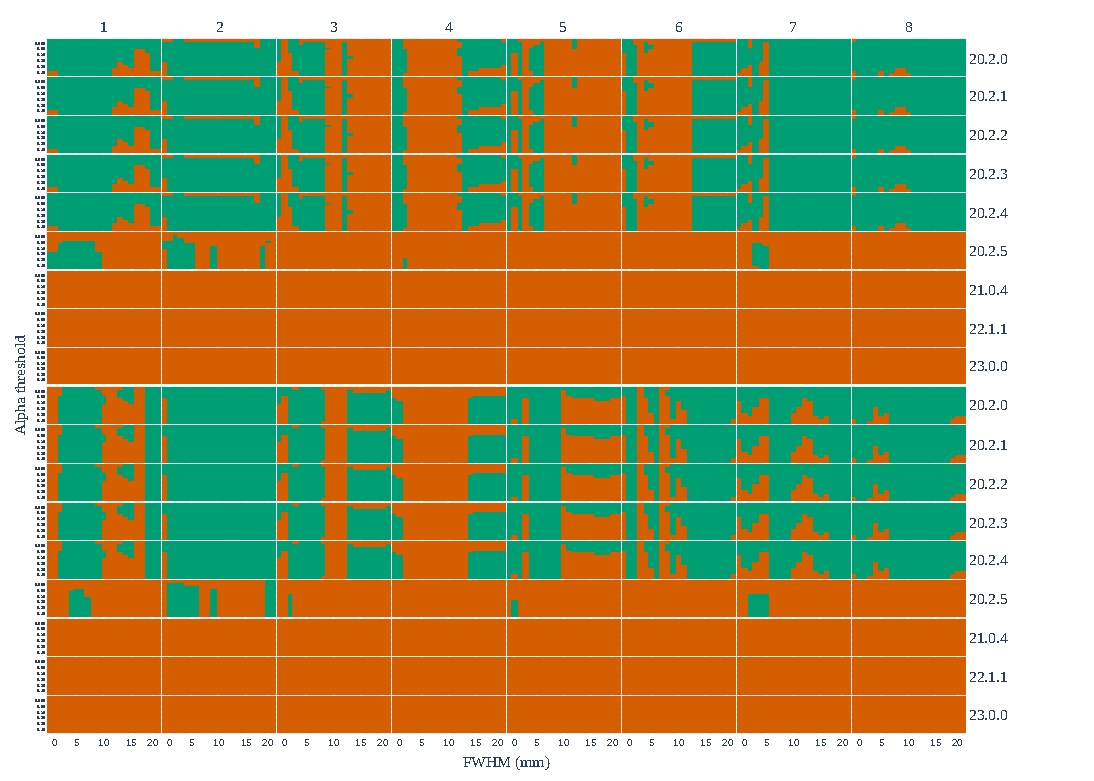
\includegraphics[width=\linewidth]{figures/fmriprep-versions/pce.pdf}
        \caption{Uncorrected test applications on different \fmriprep versions.}
        \label{fig:versions_pce}
    \end{figure}

    \begin{figure}
        \centering
        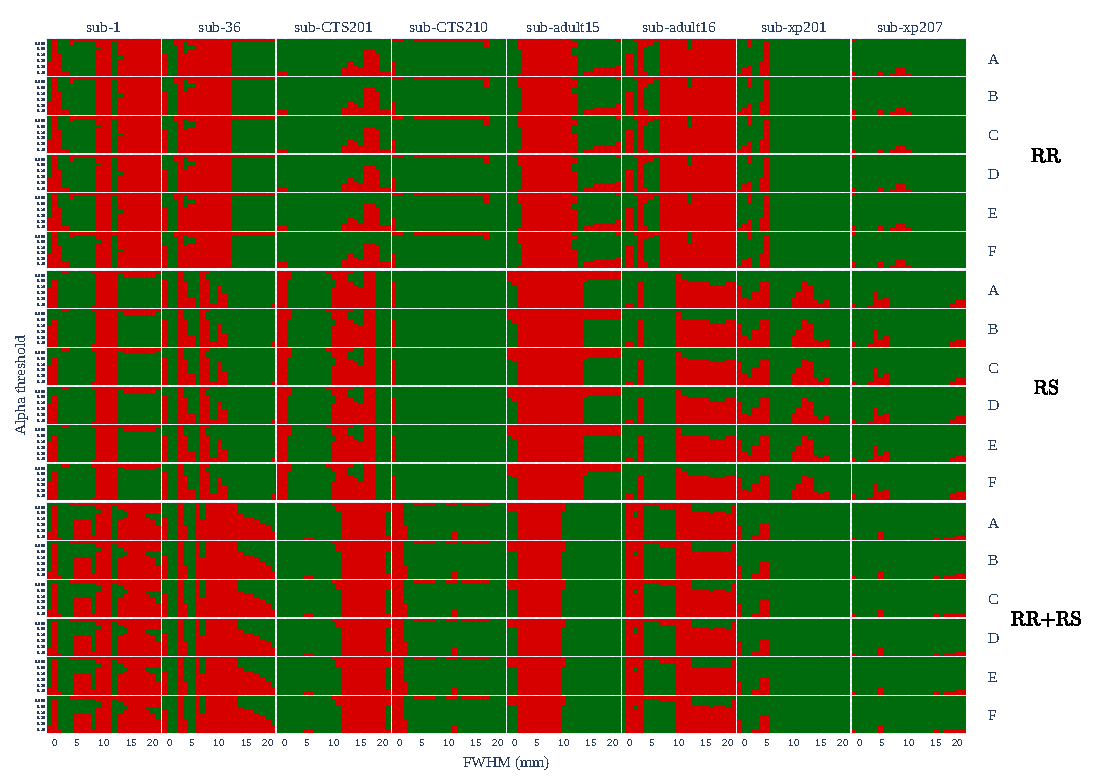
\includegraphics[width=\linewidth]{figures/arch/arch_pce_.pdf}
        \caption{Uncorrected test applications on CPU architectures.}
        \label{fig:arch_pce}
    \end{figure}


    \section{Uncertainty maps for others FWHM}

    \begin{figure}
        \centering
        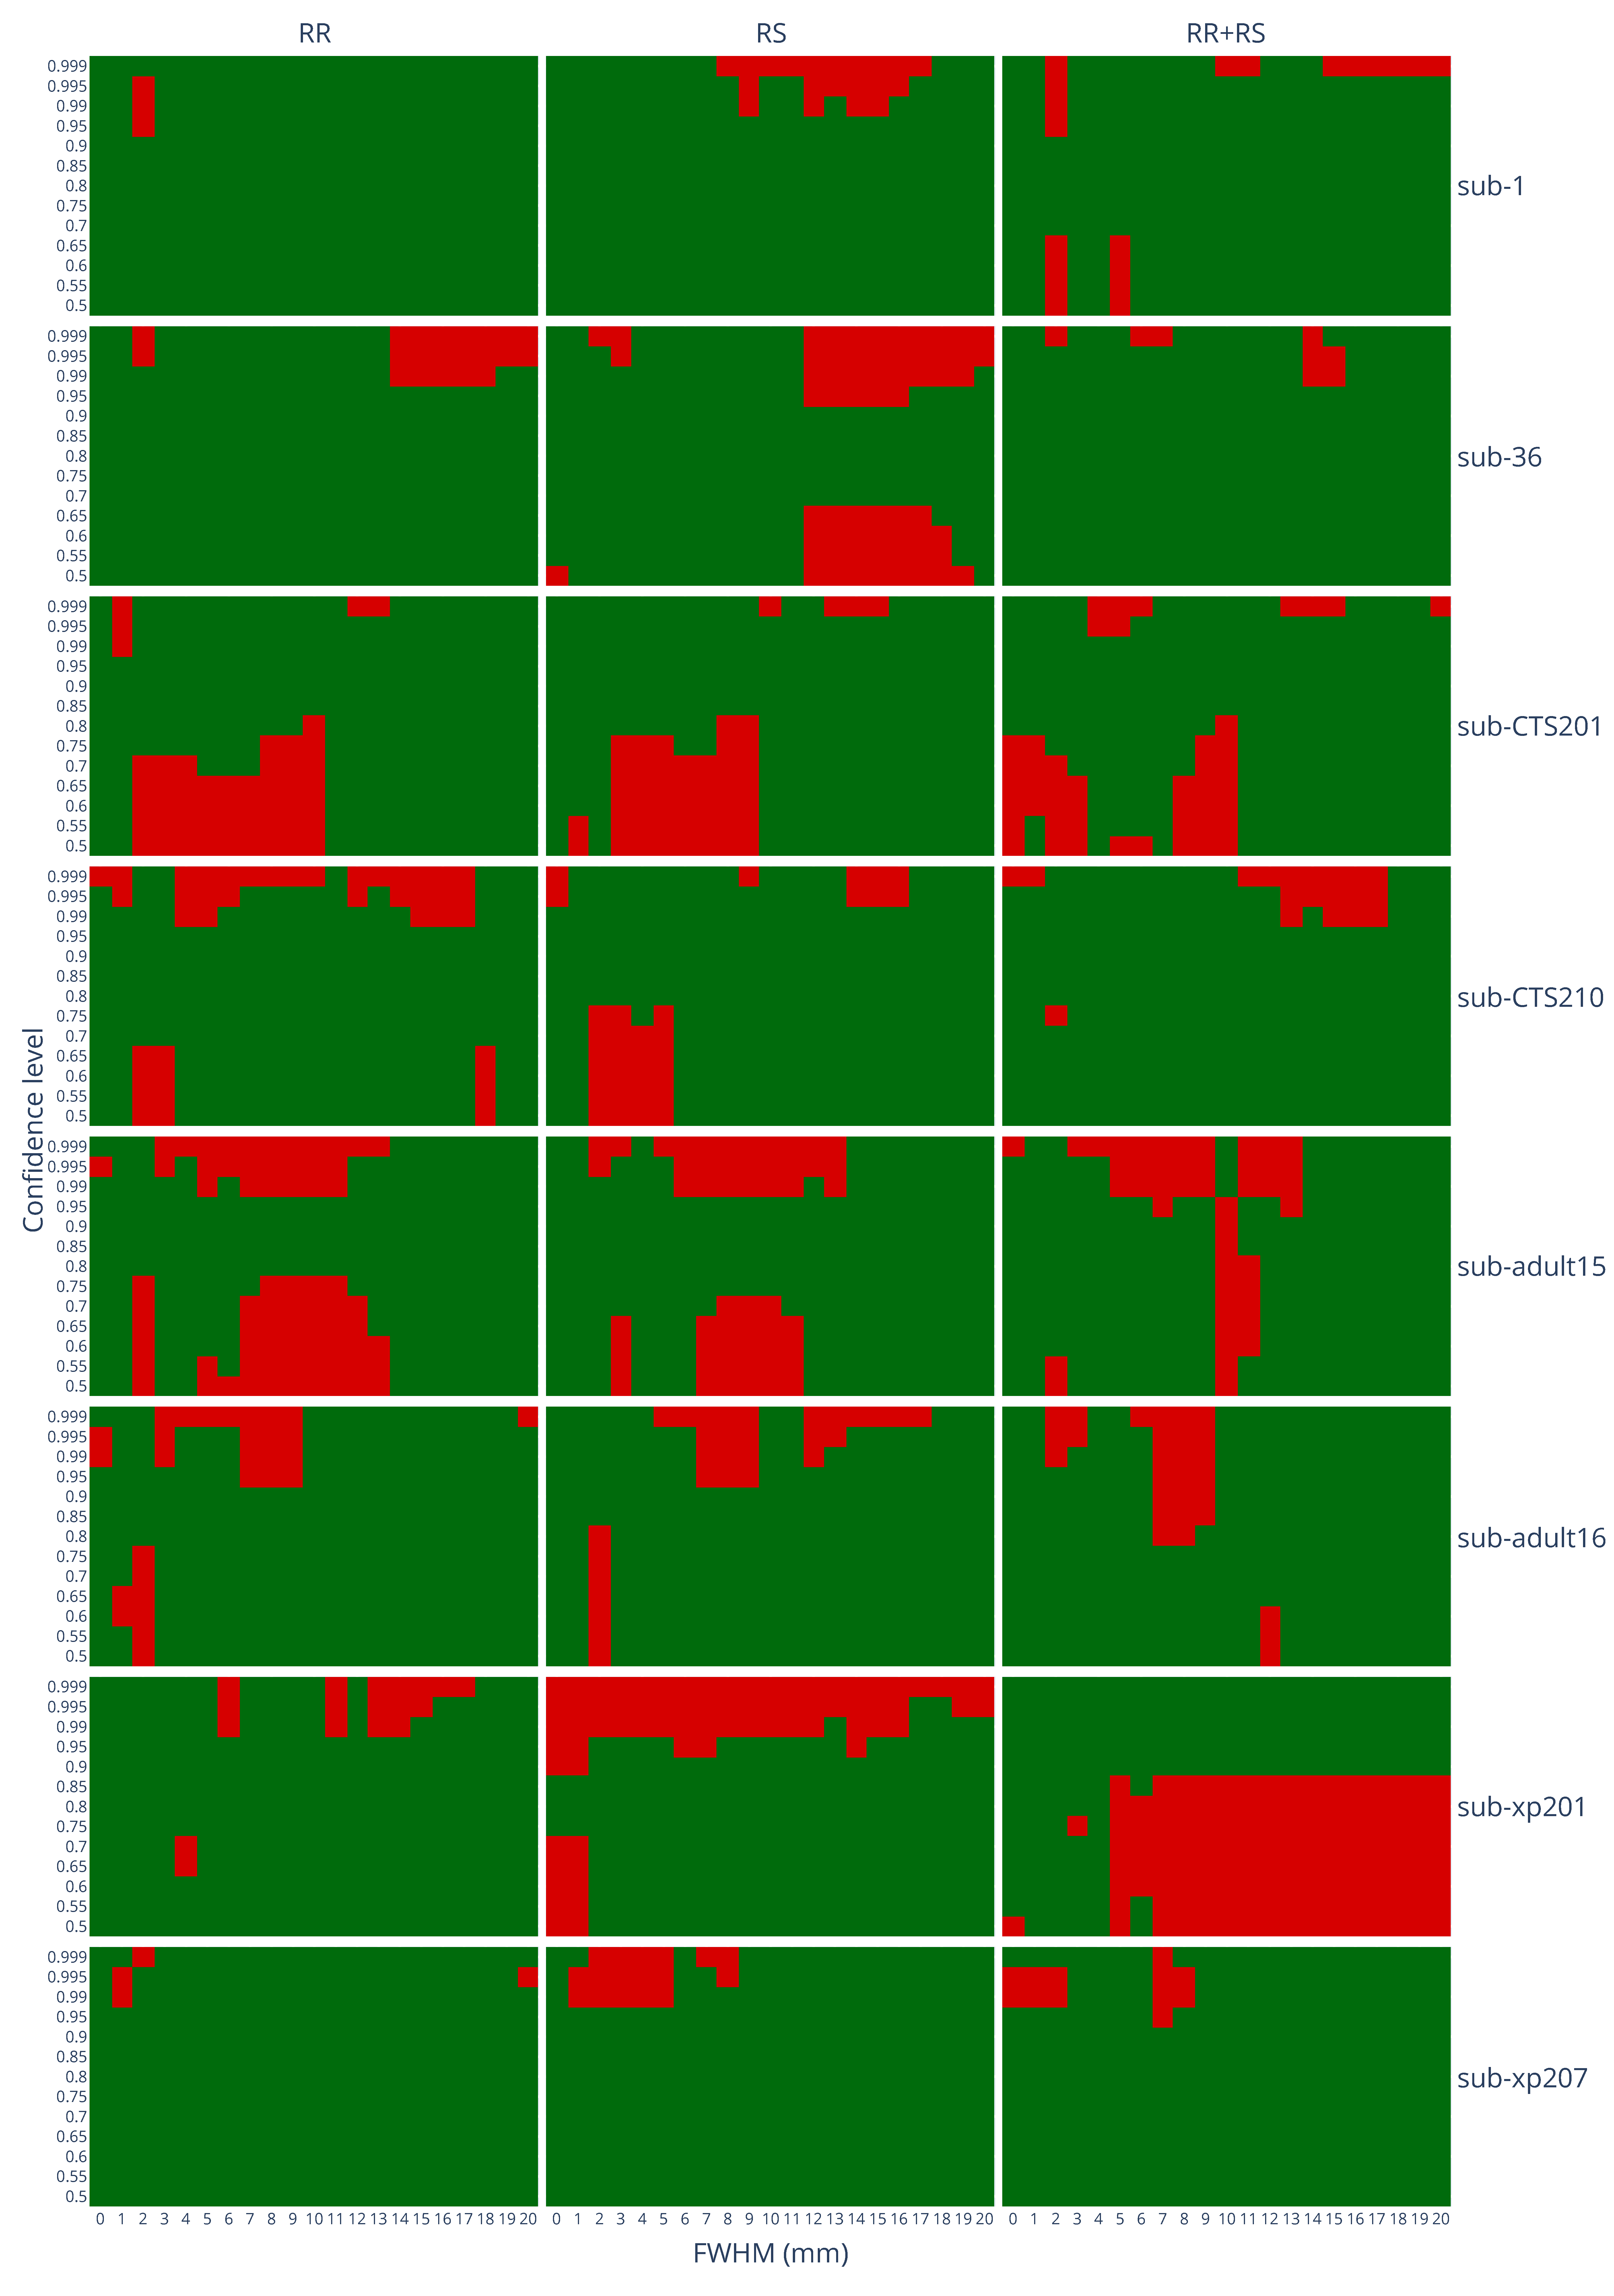
\includegraphics[width=\linewidth]{figures/exclude_pce.pdf}
        \caption{PCE}
        \label{fig:loo_pce}
    \end{figure}

    \begin{figure}
        \centering
        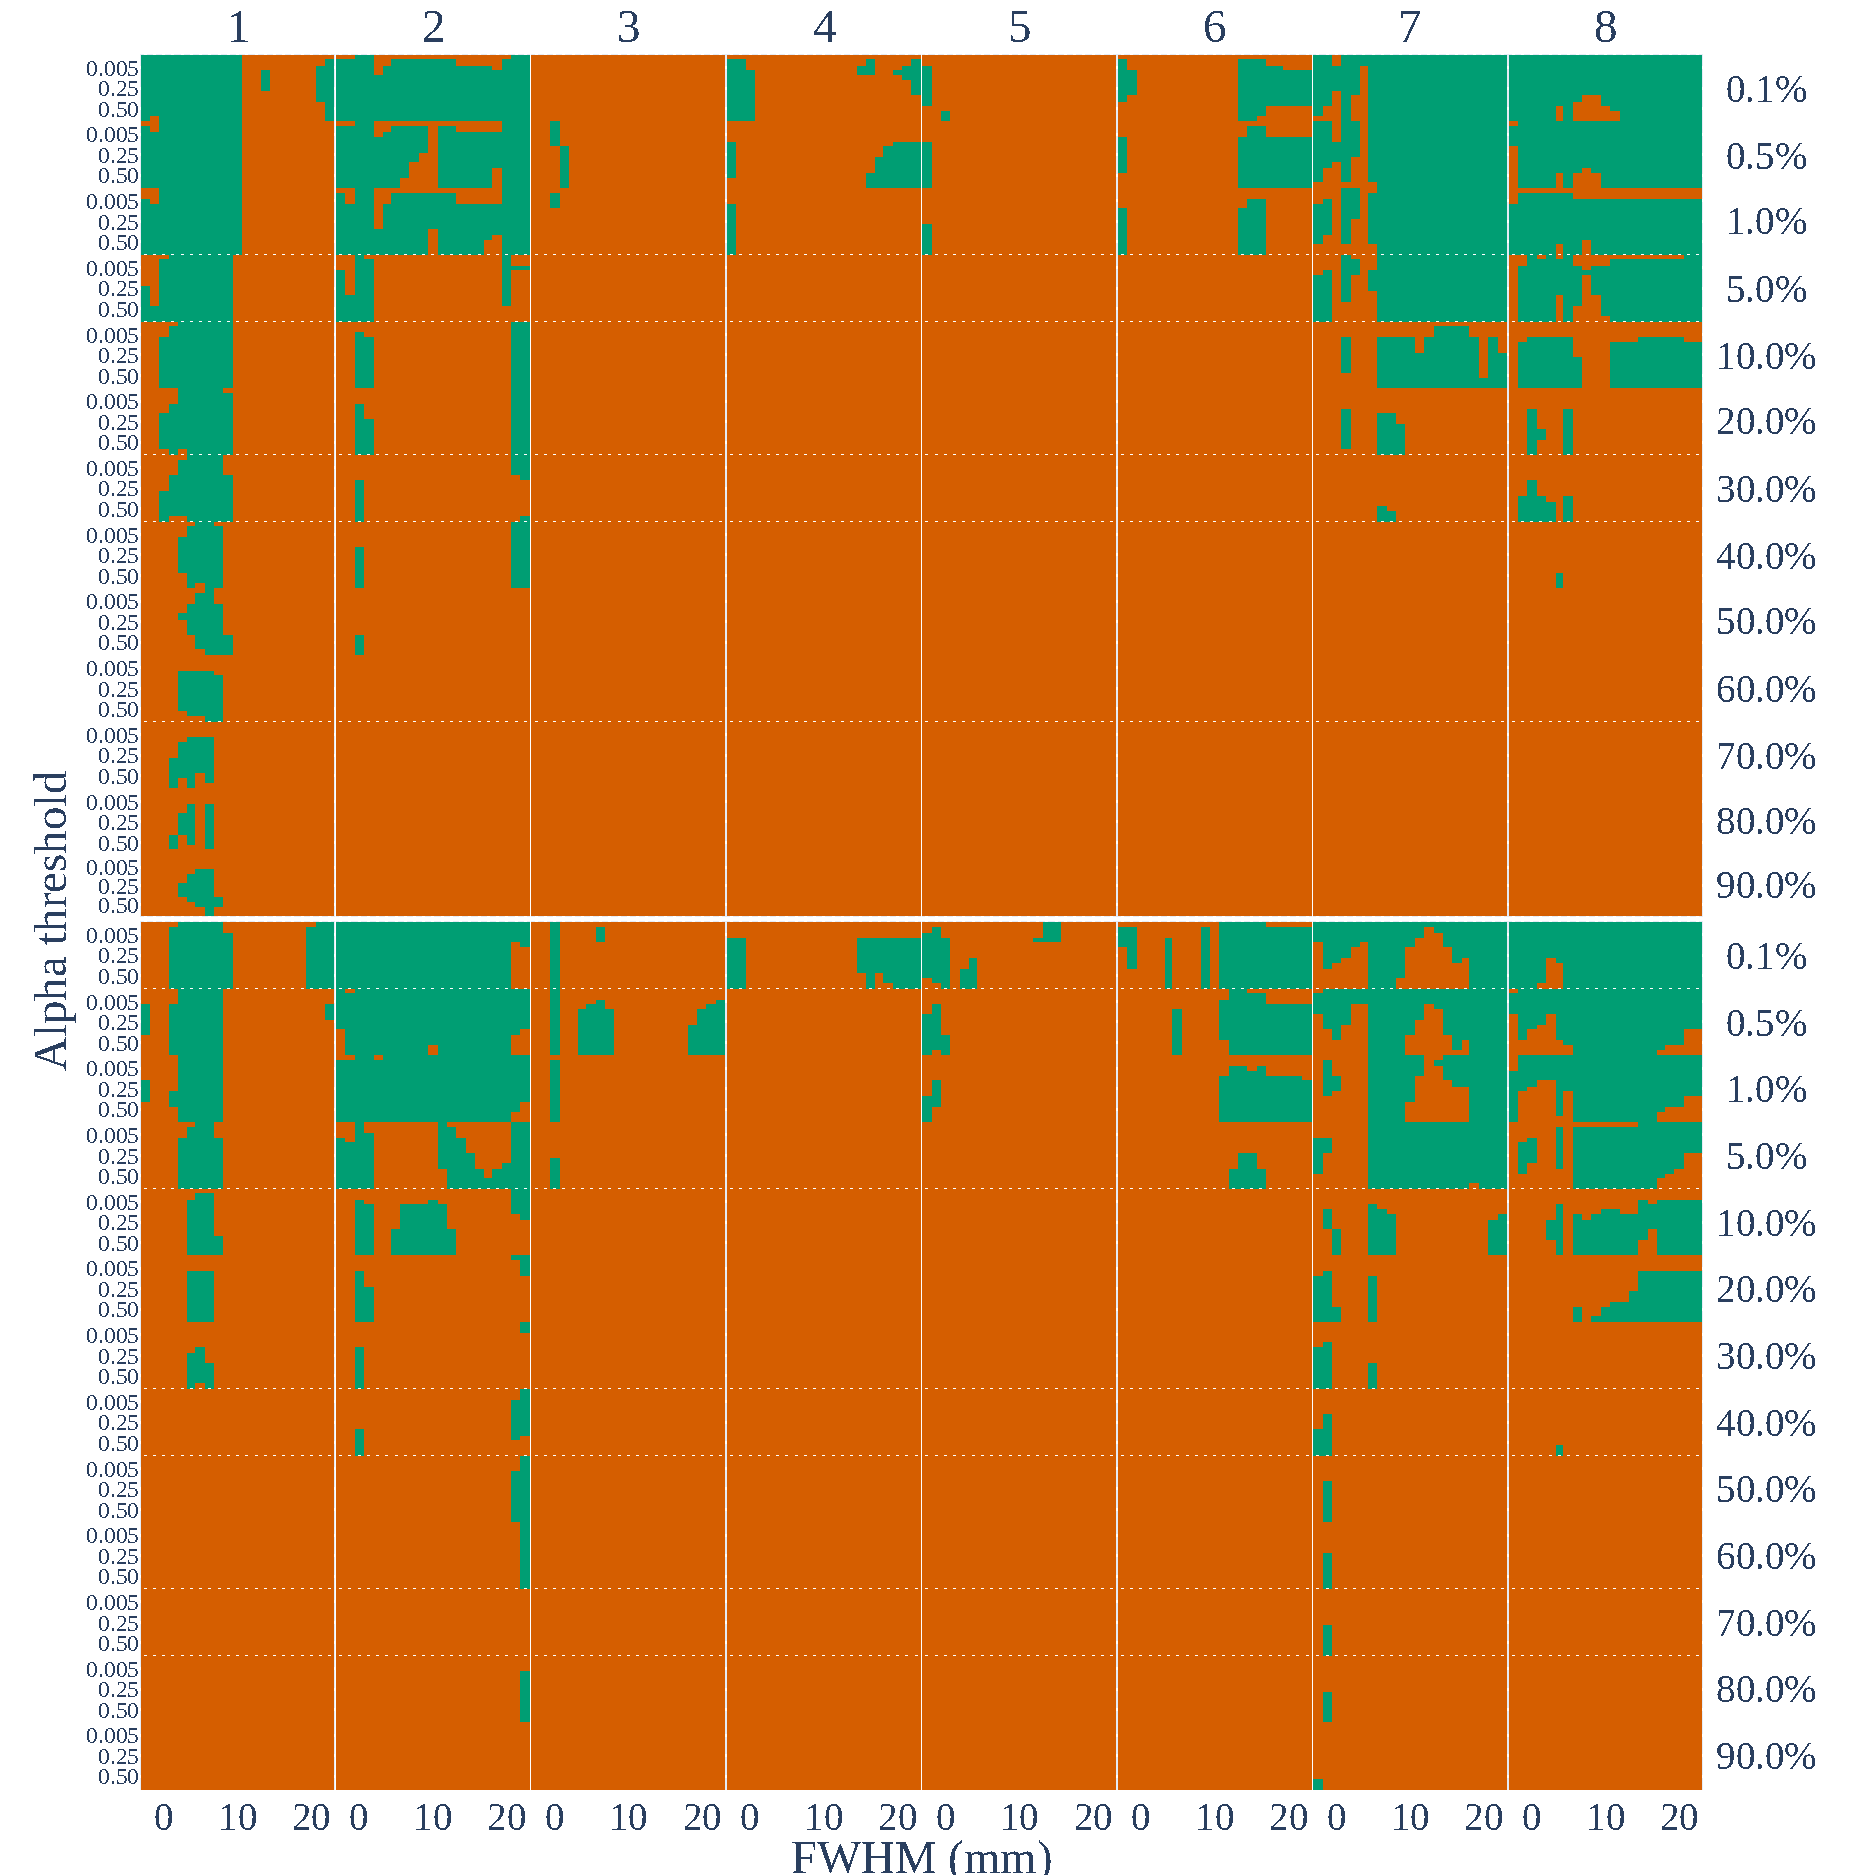
\includegraphics[width=\linewidth]{figures/template/template_pce.pdf}
        \caption{Corrupted template check for RR, RS and RR+RS mode (pce)}
    \end{figure}

    \begin{landscape}
        \begin{figure}

            \vspace*{-2cm}
            \centering
            %% sub 1
            \begin{subfigure}[b][][c]{0.01\paperwidth} 1 \vspace*{-45pt} \end{subfigure}
            \begin{subfigure}[t]{0.2\paperheight}
                \centering
                IEEE (T1 intensity)
                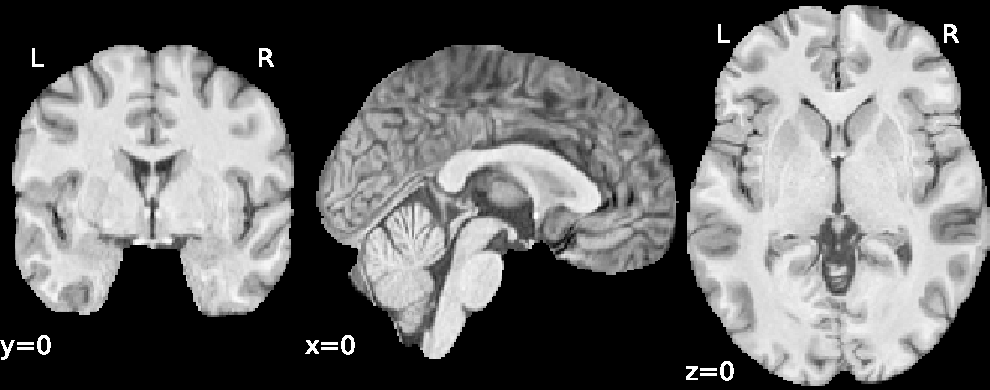
\includegraphics[width=\textwidth]{figures/sig/0mm/ieee_ds001600_sub-1.pdf}
            \end{subfigure}
            \begin{subfigure}[t]{0.2\paperheight}
                \centering
                RR (significant bits)
                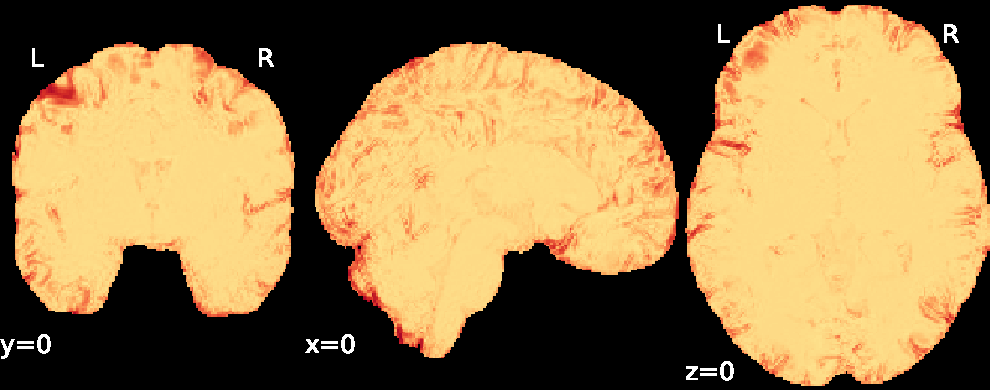
\includegraphics[width=\textwidth]{figures/sig/0mm/rr_ds001600_sub-1_sig.pdf}
            \end{subfigure}
            \begin{subfigure}[t]{0.2\paperheight}
                \centering
                RS (significant bits)
                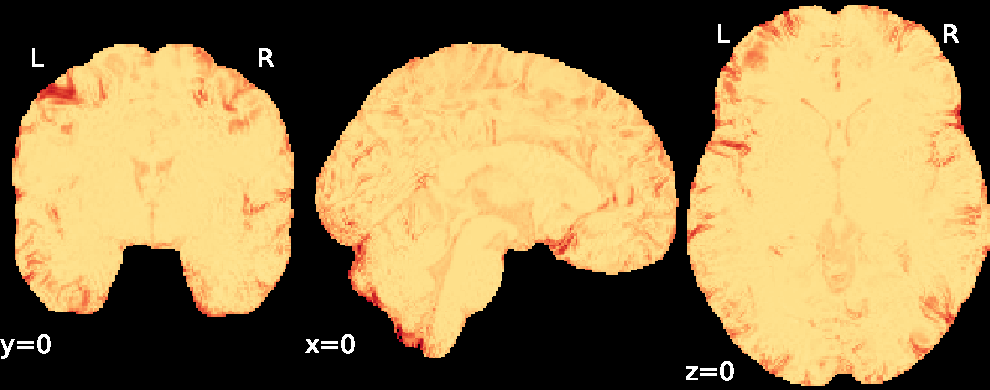
\includegraphics[width=\textwidth]{figures/sig/0mm/rs_ds001600_sub-1_sig.pdf}
            \end{subfigure}
            \begin{subfigure}[t]{0.2\paperheight}
                \centering
                RS (significant bits)
                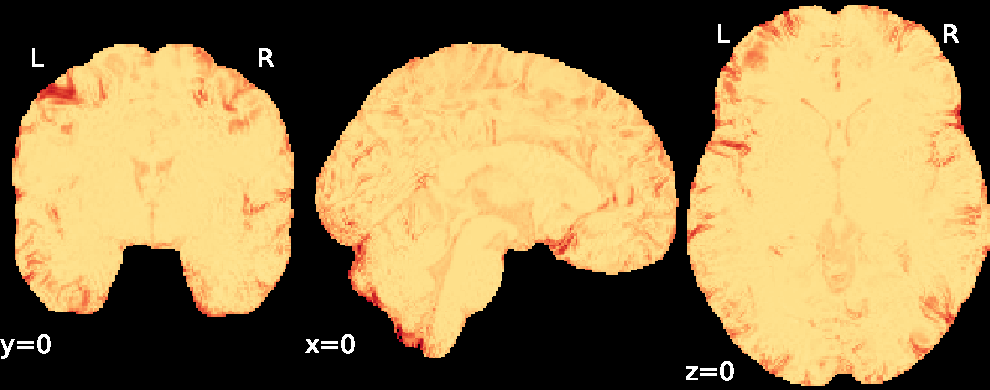
\includegraphics[width=\textwidth]{figures/sig/0mm/rs_ds001600_sub-1_sig.pdf}
            \end{subfigure} \\
            %% sub 2
            \begin{subfigure}[b][][c]{0.01\paperwidth} 2 \vspace*{15pt} \end{subfigure}
            \begin{subfigure}[t]{0.2\paperheight}
                \centering
                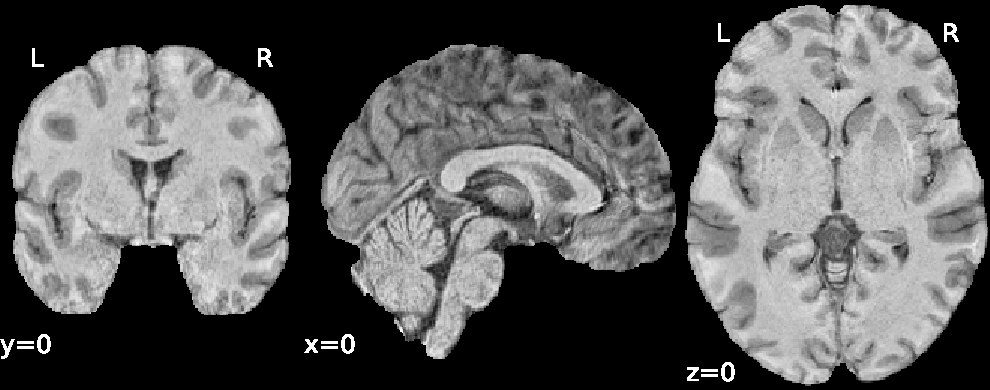
\includegraphics[width=\textwidth]{figures/sig/0mm/ieee_ds001771_sub-36.pdf}
            \end{subfigure}
            \begin{subfigure}[t]{0.2\paperheight}
                \centering
                \includegraphics[width=\textwidth]{figures/sig/0mm/rr_ds001771_sub-36_sig.pdf}
            \end{subfigure}
            \begin{subfigure}[t]{0.2\paperheight}
                \centering
                \includegraphics[width=\textwidth]{figures/sig/0mm/rs_ds001771_sub-36_sig.pdf}
            \end{subfigure}
            \begin{subfigure}[t]{0.2\paperheight}
                \centering
                \includegraphics[width=\textwidth]{figures/sig/0mm/rr.rs_ds001771_sub-36_sig.pdf}
            \end{subfigure} \\
            %% sub 3
            \begin{subfigure}[b][][c]{0.01\paperwidth} 3 \vspace*{15pt} \end{subfigure}
            \begin{subfigure}[t]{0.2\paperheight}
                \centering
                \includegraphics[width=\textwidth]{figures/sig/0mm/ieee_ds000256_sub-CTS201.pdf}
            \end{subfigure}
            \begin{subfigure}[t]{0.2\paperheight}
                \centering
                \includegraphics[width=\textwidth]{figures/sig/0mm/rr_ds000256_sub-CTS201_sig.pdf}
            \end{subfigure}
            \begin{subfigure}[t]{0.2\paperheight}
                \centering
                \includegraphics[width=\textwidth]{figures/sig/0mm/rs_ds000256_sub-CTS201_sig.pdf}
            \end{subfigure}
            \begin{subfigure}[t]{0.2\paperheight}
                \centering
                \includegraphics[width=\textwidth]{figures/sig/0mm/rr.rs_ds000256_sub-CTS201_sig.pdf}
            \end{subfigure} \\
            %% sub 4
            \begin{subfigure}[b][][c]{0.01\paperwidth} 4 \vspace*{15pt} \end{subfigure}
            \begin{subfigure}[t]{0.2\paperheight}
                \centering
                \includegraphics[width=\textwidth]{figures/sig/0mm/ieee_ds000256_sub-CTS210.pdf}
            \end{subfigure}
            \begin{subfigure}[t]{0.2\paperheight}
                \centering
                \includegraphics[width=\textwidth]{figures/sig/0mm/rr_ds000256_sub-CTS210_sig.pdf}
            \end{subfigure}
            \begin{subfigure}[t]{0.2\paperheight}
                \centering
                \includegraphics[width=\textwidth]{figures/sig/0mm/rs_ds000256_sub-CTS210_sig.pdf}
            \end{subfigure}
            \begin{subfigure}[t]{0.2\paperheight}
                \centering
                \includegraphics[width=\textwidth]{figures/sig/0mm/rr.rs_ds000256_sub-CTS210_sig.pdf}
            \end{subfigure} \\
            %% sub 5
            \begin{subfigure}[b][][c]{0.01\paperwidth} 5 \vspace*{15pt} \end{subfigure}
            \begin{subfigure}[t]{0.2\paperheight}
                \centering
                \includegraphics[width=\textwidth]{figures/sig/0mm/ieee_ds001748_sub-adult15.pdf}
            \end{subfigure}
            \begin{subfigure}[t]{0.2\paperheight}
                \centering
                \includegraphics[width=\textwidth]{figures/sig/0mm/rr_ds001748_sub-adult15_sig.pdf}
            \end{subfigure}
            \begin{subfigure}[t]{0.2\paperheight}
                \centering
                \includegraphics[width=\textwidth]{figures/sig/0mm/rs_ds001748_sub-adult15_sig.pdf}
            \end{subfigure}
            \begin{subfigure}[t]{0.2\paperheight}
                \centering
                \includegraphics[width=\textwidth]{figures/sig/0mm/rr.rs_ds001748_sub-adult15_sig.pdf}
            \end{subfigure} \\
            %% sub 6
            \begin{subfigure}[b][][c]{0.01\paperwidth} 6 \vspace*{15pt} \end{subfigure}
            \begin{subfigure}[t]{0.2\paperheight}
                \centering
                \includegraphics[width=\textwidth]{figures/sig/0mm/ieee_ds001748_sub-adult16.pdf}
            \end{subfigure}
            \begin{subfigure}[t]{0.2\paperheight}
                \centering
                \includegraphics[width=\textwidth]{figures/sig/0mm/rr_ds001748_sub-adult16_sig.pdf}
            \end{subfigure}
            \begin{subfigure}[t]{0.2\paperheight}
                \centering
                \includegraphics[width=\textwidth]{figures/sig/0mm/rs_ds001748_sub-adult16_sig.pdf}
            \end{subfigure}
            \begin{subfigure}[t]{0.2\paperheight}
                \centering
                \includegraphics[width=\textwidth]{figures/sig/0mm/rr.rs_ds001748_sub-adult16_sig.pdf}
            \end{subfigure} \\
            %% sub 7
            \begin{subfigure}[b][][c]{0.01\paperwidth} 7 \vspace*{15pt} \end{subfigure}
            \begin{subfigure}[t]{0.2\paperheight}
                \centering
                \includegraphics[width=\textwidth]{figures/sig/0mm/ieee_ds002338_sub-xp201.pdf}
            \end{subfigure}
            \begin{subfigure}[t]{0.2\paperheight}
                \centering
                \includegraphics[width=\textwidth]{figures/sig/0mm/rr_ds002338_sub-xp201_sig.pdf}
            \end{subfigure}
            \begin{subfigure}[t]{0.2\paperheight}
                \centering
                \includegraphics[width=\textwidth]{figures/sig/0mm/rs_ds002338_sub-xp201_sig.pdf}
            \end{subfigure}
            \begin{subfigure}[t]{0.2\paperheight}
                \centering
                \includegraphics[width=\textwidth]{figures/sig/0mm/rr.rs_ds002338_sub-xp201_sig.pdf}
            \end{subfigure} \\
            %% sub 8 
            \begin{subfigure}[b][][c]{0.01\paperwidth} 8 \vspace*{15pt} \end{subfigure}
            \begin{subfigure}[t]{0.2\paperheight}
                \centering
                \includegraphics[width=\textwidth]{figures/sig/0mm/ieee_ds002338_sub-xp207.pdf}
            \end{subfigure}
            \begin{subfigure}[t]{0.2\paperheight}
                \centering
                \includegraphics[width=\textwidth]{figures/sig/0mm/rr_ds002338_sub-xp207_sig.pdf}
            \end{subfigure}
            \begin{subfigure}[t]{0.2\paperheight}
                \centering
                \includegraphics[width=\textwidth]{figures/sig/0mm/rs_ds002338_sub-xp207_sig.pdf}
            \end{subfigure}
            \begin{subfigure}[t]{0.2\paperheight}
                \centering
                \includegraphics[width=\textwidth]{figures/sig/0mm/rr.rs_ds002338_sub-xp207_sig.pdf}
            \end{subfigure} \\
            \hspace*{6cm} 0 \tikz[baseline=(current bounding box.south)]{
                \draw[left color=red, right color=green!50!black, middle color=yellow]
                (0,0) rectangle (8,0.3);} 12 bits
            \caption{Uncertainty measured for subjects 1 to 8 (from top to bottom) across n=30 for
                (from right to left) IEEE, RR, RS and RR+RS perturbed samples with a spatial smoothing applied (FWHM=0mm). }
            \label{fig:uncertainty_0mm}

        \end{figure}
    \end{landscape}


    \begin{landscape}
        \begin{figure}

            \vspace*{-2cm}
            \centering
            %% sub 1
            \begin{subfigure}[b][][c]{0.01\paperwidth} 1 \vspace*{-45pt} \end{subfigure}
            \begin{subfigure}[t]{0.2\paperheight}
                \centering
                IEEE (T1 intensity)
                \includegraphics[width=\textwidth]{figures/sig/5mm/ieee_ds001600_sub-1.pdf}
            \end{subfigure}
            \begin{subfigure}[t]{0.2\paperheight}
                \centering
                RR (significant bits)
                \includegraphics[width=\textwidth]{figures/sig/5mm/rr_ds001600_sub-1_sig.pdf}
            \end{subfigure}
            \begin{subfigure}[t]{0.2\paperheight}
                \centering
                RS (significant bits)
                \includegraphics[width=\textwidth]{figures/sig/5mm/rs_ds001600_sub-1_sig.pdf}
            \end{subfigure}
            \begin{subfigure}[t]{0.2\paperheight}
                \centering
                RS (significant bits)
                \includegraphics[width=\textwidth]{figures/sig/5mm/rs_ds001600_sub-1_sig.pdf}
            \end{subfigure} \\
            %% sub 2
            \begin{subfigure}[b][][c]{0.01\paperwidth} 2 \vspace*{15pt} \end{subfigure}
            \begin{subfigure}[t]{0.2\paperheight}
                \centering
                \includegraphics[width=\textwidth]{figures/sig/5mm/ieee_ds001771_sub-36.pdf}
            \end{subfigure}
            \begin{subfigure}[t]{0.2\paperheight}
                \centering
                \includegraphics[width=\textwidth]{figures/sig/5mm/rr_ds001771_sub-36_sig.pdf}
            \end{subfigure}
            \begin{subfigure}[t]{0.2\paperheight}
                \centering
                \includegraphics[width=\textwidth]{figures/sig/5mm/rs_ds001771_sub-36_sig.pdf}
            \end{subfigure}
            \begin{subfigure}[t]{0.2\paperheight}
                \centering
                \includegraphics[width=\textwidth]{figures/sig/5mm/rr.rs_ds001771_sub-36_sig.pdf}
            \end{subfigure} \\
            %% sub 3
            \begin{subfigure}[b][][c]{0.01\paperwidth} 3 \vspace*{15pt} \end{subfigure}
            \begin{subfigure}[t]{0.2\paperheight}
                \centering
                \includegraphics[width=\textwidth]{figures/sig/5mm/ieee_ds000256_sub-CTS201.pdf}
            \end{subfigure}
            \begin{subfigure}[t]{0.2\paperheight}
                \centering
                \includegraphics[width=\textwidth]{figures/sig/5mm/rr_ds000256_sub-CTS201_sig.pdf}
            \end{subfigure}
            \begin{subfigure}[t]{0.2\paperheight}
                \centering
                \includegraphics[width=\textwidth]{figures/sig/5mm/rs_ds000256_sub-CTS201_sig.pdf}
            \end{subfigure}
            \begin{subfigure}[t]{0.2\paperheight}
                \centering
                \includegraphics[width=\textwidth]{figures/sig/5mm/rr.rs_ds000256_sub-CTS201_sig.pdf}
            \end{subfigure} \\
            %% sub 4
            \begin{subfigure}[b][][c]{0.01\paperwidth} 4 \vspace*{15pt} \end{subfigure}
            \begin{subfigure}[t]{0.2\paperheight}
                \centering
                \includegraphics[width=\textwidth]{figures/sig/5mm/ieee_ds000256_sub-CTS210.pdf}
            \end{subfigure}
            \begin{subfigure}[t]{0.2\paperheight}
                \centering
                \includegraphics[width=\textwidth]{figures/sig/5mm/rr_ds000256_sub-CTS210_sig.pdf}
            \end{subfigure}
            \begin{subfigure}[t]{0.2\paperheight}
                \centering
                \includegraphics[width=\textwidth]{figures/sig/5mm/rs_ds000256_sub-CTS210_sig.pdf}
            \end{subfigure}
            \begin{subfigure}[t]{0.2\paperheight}
                \centering
                \includegraphics[width=\textwidth]{figures/sig/5mm/rr.rs_ds000256_sub-CTS210_sig.pdf}
            \end{subfigure} \\
            %% sub 5
            \begin{subfigure}[b][][c]{0.01\paperwidth} 5 \vspace*{15pt} \end{subfigure}
            \begin{subfigure}[t]{0.2\paperheight}
                \centering
                \includegraphics[width=\textwidth]{figures/sig/5mm/ieee_ds001748_sub-adult15.pdf}
            \end{subfigure}
            \begin{subfigure}[t]{0.2\paperheight}
                \centering
                \includegraphics[width=\textwidth]{figures/sig/5mm/rr_ds001748_sub-adult15_sig.pdf}
            \end{subfigure}
            \begin{subfigure}[t]{0.2\paperheight}
                \centering
                \includegraphics[width=\textwidth]{figures/sig/5mm/rs_ds001748_sub-adult15_sig.pdf}
            \end{subfigure}
            \begin{subfigure}[t]{0.2\paperheight}
                \centering
                \includegraphics[width=\textwidth]{figures/sig/5mm/rr.rs_ds001748_sub-adult15_sig.pdf}
            \end{subfigure} \\
            %% sub 6
            \begin{subfigure}[b][][c]{0.01\paperwidth} 6 \vspace*{15pt} \end{subfigure}
            \begin{subfigure}[t]{0.2\paperheight}
                \centering
                \includegraphics[width=\textwidth]{figures/sig/5mm/ieee_ds001748_sub-adult16.pdf}
            \end{subfigure}
            \begin{subfigure}[t]{0.2\paperheight}
                \centering
                \includegraphics[width=\textwidth]{figures/sig/5mm/rr_ds001748_sub-adult16_sig.pdf}
            \end{subfigure}
            \begin{subfigure}[t]{0.2\paperheight}
                \centering
                \includegraphics[width=\textwidth]{figures/sig/5mm/rs_ds001748_sub-adult16_sig.pdf}
            \end{subfigure}
            \begin{subfigure}[t]{0.2\paperheight}
                \centering
                \includegraphics[width=\textwidth]{figures/sig/5mm/rr.rs_ds001748_sub-adult16_sig.pdf}
            \end{subfigure} \\
            %% sub 7
            \begin{subfigure}[b][][c]{0.01\paperwidth} 7 \vspace*{15pt} \end{subfigure}
            \begin{subfigure}[t]{0.2\paperheight}
                \centering
                \includegraphics[width=\textwidth]{figures/sig/5mm/ieee_ds002338_sub-xp201.pdf}
            \end{subfigure}
            \begin{subfigure}[t]{0.2\paperheight}
                \centering
                \includegraphics[width=\textwidth]{figures/sig/5mm/rr_ds002338_sub-xp201_sig.pdf}
            \end{subfigure}
            \begin{subfigure}[t]{0.2\paperheight}
                \centering
                \includegraphics[width=\textwidth]{figures/sig/5mm/rs_ds002338_sub-xp201_sig.pdf}
            \end{subfigure}
            \begin{subfigure}[t]{0.2\paperheight}
                \centering
                \includegraphics[width=\textwidth]{figures/sig/5mm/rr.rs_ds002338_sub-xp201_sig.pdf}
            \end{subfigure} \\
            %% sub 8 
            \begin{subfigure}[b][][c]{0.01\paperwidth} 8 \vspace*{15pt} \end{subfigure}
            \begin{subfigure}[t]{0.2\paperheight}
                \centering
                \includegraphics[width=\textwidth]{figures/sig/5mm/ieee_ds002338_sub-xp207.pdf}
            \end{subfigure}
            \begin{subfigure}[t]{0.2\paperheight}
                \centering
                \includegraphics[width=\textwidth]{figures/sig/5mm/rr_ds002338_sub-xp207_sig.pdf}
            \end{subfigure}
            \begin{subfigure}[t]{0.2\paperheight}
                \centering
                \includegraphics[width=\textwidth]{figures/sig/5mm/rs_ds002338_sub-xp207_sig.pdf}
            \end{subfigure}
            \begin{subfigure}[t]{0.2\paperheight}
                \centering
                \includegraphics[width=\textwidth]{figures/sig/5mm/rr.rs_ds002338_sub-xp207_sig.pdf}
            \end{subfigure} \\
            \hspace*{6cm} 0 \tikz[baseline=(current bounding box.south)]{
                \draw[left color=red, right color=green!50!black, middle color=yellow]
                (0,0) rectangle (8,0.3);} 12 bits
            \caption{Uncertainty measured for subjects 1 to 8 (from top to bottom) across n=30 for
                (from right to left) IEEE, RR, RS and RR+RS perturbed samples with a spatial smoothing applied (FWHM=5mm). }
            \label{fig:uncertainty_5mm}

        \end{figure}
    \end{landscape}


    \begin{landscape}
        \begin{figure}

            \vspace*{-2cm}
            \centering
            %% sub 1
            \begin{subfigure}[b][][c]{0.01\paperwidth} 1 \vspace*{-45pt} \end{subfigure}
            \begin{subfigure}[t]{0.2\paperheight}
                \centering
                IEEE (T1 intensity)
                \includegraphics[width=\textwidth]{figures/sig/10mm/ieee_ds001600_sub-1.pdf}
            \end{subfigure}
            \begin{subfigure}[t]{0.2\paperheight}
                \centering
                RR (significant bits)
                \includegraphics[width=\textwidth]{figures/sig/10mm/rr_ds001600_sub-1_sig.pdf}
            \end{subfigure}
            \begin{subfigure}[t]{0.2\paperheight}
                \centering
                RS (significant bits)
                \includegraphics[width=\textwidth]{figures/sig/10mm/rs_ds001600_sub-1_sig.pdf}
            \end{subfigure}
            \begin{subfigure}[t]{0.2\paperheight}
                \centering
                RS (significant bits)
                \includegraphics[width=\textwidth]{figures/sig/10mm/rs_ds001600_sub-1_sig.pdf}
            \end{subfigure} \\
            %% sub 2
            \begin{subfigure}[b][][c]{0.01\paperwidth} 2 \vspace*{15pt} \end{subfigure}
            \begin{subfigure}[t]{0.2\paperheight}
                \centering
                \includegraphics[width=\textwidth]{figures/sig/10mm/ieee_ds001771_sub-36.pdf}
            \end{subfigure}
            \begin{subfigure}[t]{0.2\paperheight}
                \centering
                \includegraphics[width=\textwidth]{figures/sig/10mm/rr_ds001771_sub-36_sig.pdf}
            \end{subfigure}
            \begin{subfigure}[t]{0.2\paperheight}
                \centering
                \includegraphics[width=\textwidth]{figures/sig/10mm/rs_ds001771_sub-36_sig.pdf}
            \end{subfigure}
            \begin{subfigure}[t]{0.2\paperheight}
                \centering
                \includegraphics[width=\textwidth]{figures/sig/10mm/rr.rs_ds001771_sub-36_sig.pdf}
            \end{subfigure} \\
            %% sub 3
            \begin{subfigure}[b][][c]{0.01\paperwidth} 3 \vspace*{15pt} \end{subfigure}
            \begin{subfigure}[t]{0.2\paperheight}
                \centering
                \includegraphics[width=\textwidth]{figures/sig/10mm/ieee_ds000256_sub-CTS201.pdf}
            \end{subfigure}
            \begin{subfigure}[t]{0.2\paperheight}
                \centering
                \includegraphics[width=\textwidth]{figures/sig/10mm/rr_ds000256_sub-CTS201_sig.pdf}
            \end{subfigure}
            \begin{subfigure}[t]{0.2\paperheight}
                \centering
                \includegraphics[width=\textwidth]{figures/sig/10mm/rs_ds000256_sub-CTS201_sig.pdf}
            \end{subfigure}
            \begin{subfigure}[t]{0.2\paperheight}
                \centering
                \includegraphics[width=\textwidth]{figures/sig/10mm/rr.rs_ds000256_sub-CTS201_sig.pdf}
            \end{subfigure} \\
            %% sub 4
            \begin{subfigure}[b][][c]{0.01\paperwidth} 4 \vspace*{15pt} \end{subfigure}
            \begin{subfigure}[t]{0.2\paperheight}
                \centering
                \includegraphics[width=\textwidth]{figures/sig/10mm/ieee_ds000256_sub-CTS210.pdf}
            \end{subfigure}
            \begin{subfigure}[t]{0.2\paperheight}
                \centering
                \includegraphics[width=\textwidth]{figures/sig/10mm/rr_ds000256_sub-CTS210_sig.pdf}
            \end{subfigure}
            \begin{subfigure}[t]{0.2\paperheight}
                \centering
                \includegraphics[width=\textwidth]{figures/sig/10mm/rs_ds000256_sub-CTS210_sig.pdf}
            \end{subfigure}
            \begin{subfigure}[t]{0.2\paperheight}
                \centering
                \includegraphics[width=\textwidth]{figures/sig/10mm/rr.rs_ds000256_sub-CTS210_sig.pdf}
            \end{subfigure} \\
            %% sub 5
            \begin{subfigure}[b][][c]{0.01\paperwidth} 5 \vspace*{15pt} \end{subfigure}
            \begin{subfigure}[t]{0.2\paperheight}
                \centering
                \includegraphics[width=\textwidth]{figures/sig/10mm/ieee_ds001748_sub-adult15.pdf}
            \end{subfigure}
            \begin{subfigure}[t]{0.2\paperheight}
                \centering
                \includegraphics[width=\textwidth]{figures/sig/10mm/rr_ds001748_sub-adult15_sig.pdf}
            \end{subfigure}
            \begin{subfigure}[t]{0.2\paperheight}
                \centering
                \includegraphics[width=\textwidth]{figures/sig/10mm/rs_ds001748_sub-adult15_sig.pdf}
            \end{subfigure}
            \begin{subfigure}[t]{0.2\paperheight}
                \centering
                \includegraphics[width=\textwidth]{figures/sig/10mm/rr.rs_ds001748_sub-adult15_sig.pdf}
            \end{subfigure} \\
            %% sub 6
            \begin{subfigure}[b][][c]{0.01\paperwidth} 6 \vspace*{15pt} \end{subfigure}
            \begin{subfigure}[t]{0.2\paperheight}
                \centering
                \includegraphics[width=\textwidth]{figures/sig/10mm/ieee_ds001748_sub-adult16.pdf}
            \end{subfigure}
            \begin{subfigure}[t]{0.2\paperheight}
                \centering
                \includegraphics[width=\textwidth]{figures/sig/10mm/rr_ds001748_sub-adult16_sig.pdf}
            \end{subfigure}
            \begin{subfigure}[t]{0.2\paperheight}
                \centering
                \includegraphics[width=\textwidth]{figures/sig/10mm/rs_ds001748_sub-adult16_sig.pdf}
            \end{subfigure}
            \begin{subfigure}[t]{0.2\paperheight}
                \centering
                \includegraphics[width=\textwidth]{figures/sig/10mm/rr.rs_ds001748_sub-adult16_sig.pdf}
            \end{subfigure} \\
            %% sub 7
            \begin{subfigure}[b][][c]{0.01\paperwidth} 7 \vspace*{15pt} \end{subfigure}
            \begin{subfigure}[t]{0.2\paperheight}
                \centering
                \includegraphics[width=\textwidth]{figures/sig/10mm/ieee_ds002338_sub-xp201.pdf}
            \end{subfigure}
            \begin{subfigure}[t]{0.2\paperheight}
                \centering
                \includegraphics[width=\textwidth]{figures/sig/10mm/rr_ds002338_sub-xp201_sig.pdf}
            \end{subfigure}
            \begin{subfigure}[t]{0.2\paperheight}
                \centering
                \includegraphics[width=\textwidth]{figures/sig/10mm/rs_ds002338_sub-xp201_sig.pdf}
            \end{subfigure}
            \begin{subfigure}[t]{0.2\paperheight}
                \centering
                \includegraphics[width=\textwidth]{figures/sig/10mm/rr.rs_ds002338_sub-xp201_sig.pdf}
            \end{subfigure} \\
            %% sub 8 
            \begin{subfigure}[b][][c]{0.01\paperwidth} 8 \vspace*{15pt} \end{subfigure}
            \begin{subfigure}[t]{0.2\paperheight}
                \centering
                \includegraphics[width=\textwidth]{figures/sig/10mm/ieee_ds002338_sub-xp207.pdf}
            \end{subfigure}
            \begin{subfigure}[t]{0.2\paperheight}
                \centering
                \includegraphics[width=\textwidth]{figures/sig/10mm/rr_ds002338_sub-xp207_sig.pdf}
            \end{subfigure}
            \begin{subfigure}[t]{0.2\paperheight}
                \centering
                \includegraphics[width=\textwidth]{figures/sig/10mm/rs_ds002338_sub-xp207_sig.pdf}
            \end{subfigure}
            \begin{subfigure}[t]{0.2\paperheight}
                \centering
                \includegraphics[width=\textwidth]{figures/sig/10mm/rr.rs_ds002338_sub-xp207_sig.pdf}
            \end{subfigure} \\
            \hspace*{6cm} 0 \tikz[baseline=(current bounding box.south)]{
                \draw[left color=red, right color=green!50!black, middle color=yellow]
                (0,0) rectangle (8,0.3);} 12 bits
            \caption{Uncertainty measured for subjects 1 to 8 (from top to bottom) across n=30 for
                (from right to left) IEEE, RR, RS and RR+RS perturbed samples with a spatial smoothing applied (FWHM=10mm). }
            \label{fig:uncertainty_10mm}

        \end{figure}
    \end{landscape}

    \begin{landscape}
        \begin{figure}

            \vspace*{-2cm}
            \centering
            %% sub 1
            \begin{subfigure}[b][][c]{0.01\paperwidth} 1 \vspace*{-45pt} \end{subfigure}
            \begin{subfigure}[t]{0.2\paperheight}
                \centering
                IEEE (T1 intensity)
                \includegraphics[width=\textwidth]{figures/sig/15mm/ieee_ds001600_sub-1.pdf}
            \end{subfigure}
            \begin{subfigure}[t]{0.2\paperheight}
                \centering
                RR (significant bits)
                \includegraphics[width=\textwidth]{figures/sig/15mm/rr_ds001600_sub-1_sig.pdf}
            \end{subfigure}
            \begin{subfigure}[t]{0.2\paperheight}
                \centering
                RS (significant bits)
                \includegraphics[width=\textwidth]{figures/sig/15mm/rs_ds001600_sub-1_sig.pdf}
            \end{subfigure}
            \begin{subfigure}[t]{0.2\paperheight}
                \centering
                RS (significant bits)
                \includegraphics[width=\textwidth]{figures/sig/15mm/rs_ds001600_sub-1_sig.pdf}
            \end{subfigure} \\
            %% sub 2
            \begin{subfigure}[b][][c]{0.01\paperwidth} 2 \vspace*{15pt} \end{subfigure}
            \begin{subfigure}[t]{0.2\paperheight}
                \centering
                \includegraphics[width=\textwidth]{figures/sig/15mm/ieee_ds001771_sub-36.pdf}
            \end{subfigure}
            \begin{subfigure}[t]{0.2\paperheight}
                \centering
                \includegraphics[width=\textwidth]{figures/sig/15mm/rr_ds001771_sub-36_sig.pdf}
            \end{subfigure}
            \begin{subfigure}[t]{0.2\paperheight}
                \centering
                \includegraphics[width=\textwidth]{figures/sig/15mm/rs_ds001771_sub-36_sig.pdf}
            \end{subfigure}
            \begin{subfigure}[t]{0.2\paperheight}
                \centering
                \includegraphics[width=\textwidth]{figures/sig/15mm/rr.rs_ds001771_sub-36_sig.pdf}
            \end{subfigure} \\
            %% sub 3
            \begin{subfigure}[b][][c]{0.01\paperwidth} 3 \vspace*{15pt} \end{subfigure}
            \begin{subfigure}[t]{0.2\paperheight}
                \centering
                \includegraphics[width=\textwidth]{figures/sig/15mm/ieee_ds000256_sub-CTS201.pdf}
            \end{subfigure}
            \begin{subfigure}[t]{0.2\paperheight}
                \centering
                \includegraphics[width=\textwidth]{figures/sig/15mm/rr_ds000256_sub-CTS201_sig.pdf}
            \end{subfigure}
            \begin{subfigure}[t]{0.2\paperheight}
                \centering
                \includegraphics[width=\textwidth]{figures/sig/15mm/rs_ds000256_sub-CTS201_sig.pdf}
            \end{subfigure}
            \begin{subfigure}[t]{0.2\paperheight}
                \centering
                \includegraphics[width=\textwidth]{figures/sig/15mm/rr.rs_ds000256_sub-CTS201_sig.pdf}
            \end{subfigure} \\
            %% sub 4
            \begin{subfigure}[b][][c]{0.01\paperwidth} 4 \vspace*{15pt} \end{subfigure}
            \begin{subfigure}[t]{0.2\paperheight}
                \centering
                \includegraphics[width=\textwidth]{figures/sig/15mm/ieee_ds000256_sub-CTS210.pdf}
            \end{subfigure}
            \begin{subfigure}[t]{0.2\paperheight}
                \centering
                \includegraphics[width=\textwidth]{figures/sig/15mm/rr_ds000256_sub-CTS210_sig.pdf}
            \end{subfigure}
            \begin{subfigure}[t]{0.2\paperheight}
                \centering
                \includegraphics[width=\textwidth]{figures/sig/15mm/rs_ds000256_sub-CTS210_sig.pdf}
            \end{subfigure}
            \begin{subfigure}[t]{0.2\paperheight}
                \centering
                \includegraphics[width=\textwidth]{figures/sig/15mm/rr.rs_ds000256_sub-CTS210_sig.pdf}
            \end{subfigure} \\
            %% sub 5
            \begin{subfigure}[b][][c]{0.01\paperwidth} 5 \vspace*{15pt} \end{subfigure}
            \begin{subfigure}[t]{0.2\paperheight}
                \centering
                \includegraphics[width=\textwidth]{figures/sig/15mm/ieee_ds001748_sub-adult15.pdf}
            \end{subfigure}
            \begin{subfigure}[t]{0.2\paperheight}
                \centering
                \includegraphics[width=\textwidth]{figures/sig/15mm/rr_ds001748_sub-adult15_sig.pdf}
            \end{subfigure}
            \begin{subfigure}[t]{0.2\paperheight}
                \centering
                \includegraphics[width=\textwidth]{figures/sig/15mm/rs_ds001748_sub-adult15_sig.pdf}
            \end{subfigure}
            \begin{subfigure}[t]{0.2\paperheight}
                \centering
                \includegraphics[width=\textwidth]{figures/sig/15mm/rr.rs_ds001748_sub-adult15_sig.pdf}
            \end{subfigure} \\
            %% sub 6
            \begin{subfigure}[b][][c]{0.01\paperwidth} 6 \vspace*{15pt} \end{subfigure}
            \begin{subfigure}[t]{0.2\paperheight}
                \centering
                \includegraphics[width=\textwidth]{figures/sig/15mm/ieee_ds001748_sub-adult16.pdf}
            \end{subfigure}
            \begin{subfigure}[t]{0.2\paperheight}
                \centering
                \includegraphics[width=\textwidth]{figures/sig/15mm/rr_ds001748_sub-adult16_sig.pdf}
            \end{subfigure}
            \begin{subfigure}[t]{0.2\paperheight}
                \centering
                \includegraphics[width=\textwidth]{figures/sig/15mm/rs_ds001748_sub-adult16_sig.pdf}
            \end{subfigure}
            \begin{subfigure}[t]{0.2\paperheight}
                \centering
                \includegraphics[width=\textwidth]{figures/sig/15mm/rr.rs_ds001748_sub-adult16_sig.pdf}
            \end{subfigure} \\
            %% sub 7
            \begin{subfigure}[b][][c]{0.01\paperwidth} 7 \vspace*{15pt} \end{subfigure}
            \begin{subfigure}[t]{0.2\paperheight}
                \centering
                \includegraphics[width=\textwidth]{figures/sig/15mm/ieee_ds002338_sub-xp201.pdf}
            \end{subfigure}
            \begin{subfigure}[t]{0.2\paperheight}
                \centering
                \includegraphics[width=\textwidth]{figures/sig/15mm/rr_ds002338_sub-xp201_sig.pdf}
            \end{subfigure}
            \begin{subfigure}[t]{0.2\paperheight}
                \centering
                \includegraphics[width=\textwidth]{figures/sig/15mm/rs_ds002338_sub-xp201_sig.pdf}
            \end{subfigure}
            \begin{subfigure}[t]{0.2\paperheight}
                \centering
                \includegraphics[width=\textwidth]{figures/sig/15mm/rr.rs_ds002338_sub-xp201_sig.pdf}
            \end{subfigure} \\
            %% sub 8 
            \begin{subfigure}[b][][c]{0.01\paperwidth} 8 \vspace*{15pt} \end{subfigure}
            \begin{subfigure}[t]{0.2\paperheight}
                \centering
                \includegraphics[width=\textwidth]{figures/sig/15mm/ieee_ds002338_sub-xp207.pdf}
            \end{subfigure}
            \begin{subfigure}[t]{0.2\paperheight}
                \centering
                \includegraphics[width=\textwidth]{figures/sig/15mm/rr_ds002338_sub-xp207_sig.pdf}
            \end{subfigure}
            \begin{subfigure}[t]{0.2\paperheight}
                \centering
                \includegraphics[width=\textwidth]{figures/sig/15mm/rs_ds002338_sub-xp207_sig.pdf}
            \end{subfigure}
            \begin{subfigure}[t]{0.2\paperheight}
                \centering
                \includegraphics[width=\textwidth]{figures/sig/15mm/rr.rs_ds002338_sub-xp207_sig.pdf}
            \end{subfigure} \\
            \hspace*{6cm} 0 \tikz[baseline=(current bounding box.south)]{
                \draw[left color=red, right color=green!50!black, middle color=yellow]
                (0,0) rectangle (8,0.3);} 12 bits
            \caption{Uncertainty measured for subjects 1 to 8 (from top to bottom) across n=30 for
                (from right to left) IEEE, RR, RS and RR+RS perturbed samples with a spatial smoothing applied (FWHM=15mm). }
            \label{fig:uncertainty_15mm}

        \end{figure}
    \end{landscape}

    \begin{landscape}
        \begin{figure}

            \vspace*{-2cm}
            \centering
            %% sub 1
            \begin{subfigure}[b][][c]{0.01\paperwidth} 1 \vspace*{-45pt} \end{subfigure}
            \begin{subfigure}[t]{0.2\paperheight}
                \centering
                IEEE (T1 intensity)
                \includegraphics[width=\textwidth]{figures/sig/20mm/ieee_ds001600_sub-1.pdf}
            \end{subfigure}
            \begin{subfigure}[t]{0.2\paperheight}
                \centering
                RR (significant bits)
                \includegraphics[width=\textwidth]{figures/sig/20mm/rr_ds001600_sub-1_sig.pdf}
            \end{subfigure}
            \begin{subfigure}[t]{0.2\paperheight}
                \centering
                RS (significant bits)
                \includegraphics[width=\textwidth]{figures/sig/20mm/rs_ds001600_sub-1_sig.pdf}
            \end{subfigure}
            \begin{subfigure}[t]{0.2\paperheight}
                \centering
                RS (significant bits)
                \includegraphics[width=\textwidth]{figures/sig/20mm/rs_ds001600_sub-1_sig.pdf}
            \end{subfigure} \\
            %% sub 2
            \begin{subfigure}[b][][c]{0.01\paperwidth} 2 \vspace*{15pt} \end{subfigure}
            \begin{subfigure}[t]{0.2\paperheight}
                \centering
                \includegraphics[width=\textwidth]{figures/sig/20mm/ieee_ds001771_sub-36.pdf}
            \end{subfigure}
            \begin{subfigure}[t]{0.2\paperheight}
                \centering
                \includegraphics[width=\textwidth]{figures/sig/20mm/rr_ds001771_sub-36_sig.pdf}
            \end{subfigure}
            \begin{subfigure}[t]{0.2\paperheight}
                \centering
                \includegraphics[width=\textwidth]{figures/sig/20mm/rs_ds001771_sub-36_sig.pdf}
            \end{subfigure}
            \begin{subfigure}[t]{0.2\paperheight}
                \centering
                \includegraphics[width=\textwidth]{figures/sig/20mm/rr.rs_ds001771_sub-36_sig.pdf}
            \end{subfigure} \\
            %% sub 3
            \begin{subfigure}[b][][c]{0.01\paperwidth} 3 \vspace*{15pt} \end{subfigure}
            \begin{subfigure}[t]{0.2\paperheight}
                \centering
                \includegraphics[width=\textwidth]{figures/sig/20mm/ieee_ds000256_sub-CTS201.pdf}
            \end{subfigure}
            \begin{subfigure}[t]{0.2\paperheight}
                \centering
                \includegraphics[width=\textwidth]{figures/sig/20mm/rr_ds000256_sub-CTS201_sig.pdf}
            \end{subfigure}
            \begin{subfigure}[t]{0.2\paperheight}
                \centering
                \includegraphics[width=\textwidth]{figures/sig/20mm/rs_ds000256_sub-CTS201_sig.pdf}
            \end{subfigure}
            \begin{subfigure}[t]{0.2\paperheight}
                \centering
                \includegraphics[width=\textwidth]{figures/sig/20mm/rr.rs_ds000256_sub-CTS201_sig.pdf}
            \end{subfigure} \\
            %% sub 4
            \begin{subfigure}[b][][c]{0.01\paperwidth} 4 \vspace*{15pt} \end{subfigure}
            \begin{subfigure}[t]{0.2\paperheight}
                \centering
                \includegraphics[width=\textwidth]{figures/sig/20mm/ieee_ds000256_sub-CTS210.pdf}
            \end{subfigure}
            \begin{subfigure}[t]{0.2\paperheight}
                \centering
                \includegraphics[width=\textwidth]{figures/sig/20mm/rr_ds000256_sub-CTS210_sig.pdf}
            \end{subfigure}
            \begin{subfigure}[t]{0.2\paperheight}
                \centering
                \includegraphics[width=\textwidth]{figures/sig/20mm/rs_ds000256_sub-CTS210_sig.pdf}
            \end{subfigure}
            \begin{subfigure}[t]{0.2\paperheight}
                \centering
                \includegraphics[width=\textwidth]{figures/sig/20mm/rr.rs_ds000256_sub-CTS210_sig.pdf}
            \end{subfigure} \\
            %% sub 5
            \begin{subfigure}[b][][c]{0.01\paperwidth} 5 \vspace*{15pt} \end{subfigure}
            \begin{subfigure}[t]{0.2\paperheight}
                \centering
                \includegraphics[width=\textwidth]{figures/sig/20mm/ieee_ds001748_sub-adult15.pdf}
            \end{subfigure}
            \begin{subfigure}[t]{0.2\paperheight}
                \centering
                \includegraphics[width=\textwidth]{figures/sig/20mm/rr_ds001748_sub-adult15_sig.pdf}
            \end{subfigure}
            \begin{subfigure}[t]{0.2\paperheight}
                \centering
                \includegraphics[width=\textwidth]{figures/sig/20mm/rs_ds001748_sub-adult15_sig.pdf}
            \end{subfigure}
            \begin{subfigure}[t]{0.2\paperheight}
                \centering
                \includegraphics[width=\textwidth]{figures/sig/20mm/rr.rs_ds001748_sub-adult15_sig.pdf}
            \end{subfigure} \\
            %% sub 6
            \begin{subfigure}[b][][c]{0.01\paperwidth} 6 \vspace*{15pt} \end{subfigure}
            \begin{subfigure}[t]{0.2\paperheight}
                \centering
                \includegraphics[width=\textwidth]{figures/sig/20mm/ieee_ds001748_sub-adult16.pdf}
            \end{subfigure}
            \begin{subfigure}[t]{0.2\paperheight}
                \centering
                \includegraphics[width=\textwidth]{figures/sig/20mm/rr_ds001748_sub-adult16_sig.pdf}
            \end{subfigure}
            \begin{subfigure}[t]{0.2\paperheight}
                \centering
                \includegraphics[width=\textwidth]{figures/sig/20mm/rs_ds001748_sub-adult16_sig.pdf}
            \end{subfigure}
            \begin{subfigure}[t]{0.2\paperheight}
                \centering
                \includegraphics[width=\textwidth]{figures/sig/20mm/rr.rs_ds001748_sub-adult16_sig.pdf}
            \end{subfigure} \\
            %% sub 7
            \begin{subfigure}[b][][c]{0.01\paperwidth} 7 \vspace*{15pt} \end{subfigure}
            \begin{subfigure}[t]{0.2\paperheight}
                \centering
                \includegraphics[width=\textwidth]{figures/sig/20mm/ieee_ds002338_sub-xp201.pdf}
            \end{subfigure}
            \begin{subfigure}[t]{0.2\paperheight}
                \centering
                \includegraphics[width=\textwidth]{figures/sig/20mm/rr_ds002338_sub-xp201_sig.pdf}
            \end{subfigure}
            \begin{subfigure}[t]{0.2\paperheight}
                \centering
                \includegraphics[width=\textwidth]{figures/sig/20mm/rs_ds002338_sub-xp201_sig.pdf}
            \end{subfigure}
            \begin{subfigure}[t]{0.2\paperheight}
                \centering
                \includegraphics[width=\textwidth]{figures/sig/20mm/rr.rs_ds002338_sub-xp201_sig.pdf}
            \end{subfigure} \\
            %% sub 8 
            \begin{subfigure}[b][][c]{0.01\paperwidth} 8 \vspace*{15pt} \end{subfigure}
            \begin{subfigure}[t]{0.2\paperheight}
                \centering
                \includegraphics[width=\textwidth]{figures/sig/20mm/ieee_ds002338_sub-xp207.pdf}
            \end{subfigure}
            \begin{subfigure}[t]{0.2\paperheight}
                \centering
                \includegraphics[width=\textwidth]{figures/sig/20mm/rr_ds002338_sub-xp207_sig.pdf}
            \end{subfigure}
            \begin{subfigure}[t]{0.2\paperheight}
                \centering
                \includegraphics[width=\textwidth]{figures/sig/20mm/rs_ds002338_sub-xp207_sig.pdf}
            \end{subfigure}
            \begin{subfigure}[t]{0.2\paperheight}
                \centering
                \includegraphics[width=\textwidth]{figures/sig/20mm/rr.rs_ds002338_sub-xp207_sig.pdf}
            \end{subfigure} \\
            \hspace*{6cm} 0 \tikz[baseline=(current bounding box.south)]{
                \draw[left color=red, right color=green!50!black, middle color=yellow]
                (0,0) rectangle (8,0.3);} 12 bits
            \caption{Uncertainty measured for subjects 1 to 8 (from top to bottom) across n=30 for
                (from right to left) IEEE, RR, RS and RR+RS perturbed samples with a spatial smoothing applied (FWHM=20mm). }
            \label{fig:uncertainty_20mm}

        \end{figure}
    \end{landscape}


    \section*{Summary \fmriprep versions}

    \begin{itemize}
        \item 20.2.0: first fMRIPrep LTS (long-term support)
        \item 20.2.1:
              \begin{itemize}
                  \item ENH: Output TaskName and timing metadata for all resampled BOLD series (2320)
                  \item ENH: Add --output-layout CLI option to enable BIDS (YODA) mode (2303)
                  \item ENH: Add Docker authentication to increase pull rate limit (2316)
                  \item FIX: Specify logger for warning (2298)
              \end{itemize}
        \item 20.2.2:
              \begin{itemize}
                  \item FIX: Feed NiTransforms with LTAs of type RAS2RAS (2444)
                  \item FIX: Add some clarity to BrokenProcessPool failures (2436)
                  \item FIX: Fall-back to initializing workflow in main process (2435)
                  \item FIX: Raise informative error when duplicate subworkflows are added (2434)
                  \item FIX: Non-existing path or JSON syntax error for --bids-filter-file should raise on error (2331)
                  \item FIX: Ignore SBRef files if --ignore sbref is passed (2370)
                  \item ENH: Relax requirement for PyBIDS databases to exist (2429)
                  \item ENH: Improve \_get\_series\_len performance (2406)
                  \item ENH: Set and track NumPy's random seed (2400)
                  \item DOC: Skull-stripping is forced by default (2430)
                  \item MAINT: Pin nilearn==0.6.2 (2427)
                  \item MAINT: Pin tedana==0.0.9a1 for LTS branch (2403)
                  \item MAINT: Failing CI (2401)
              \end{itemize}
        \item 20.2.3:
              \begin{itemize}
                  \item FIX: Address the problems of a sloppy merge (2468)
                  \item FIX: DerivativesDataSink nondeterministic checksums fixed with niworkflows=~1.3.4 (2458)
                  \item FIX: Address dependency incompatibilities by pinning specific packages (2463)
                  \item FIX: Unprotected import of sentry\_sdk, which is not a dependency (2460)
                  \item ENH: Detect 3D Acknowledgments too-short BOLD series, warn and skip run's workflow building (2461)
                  \item DOC: Transfer duplicated documentation to www.nipreps.org (2469)
                  \item DOC: Better explanation on how spike regressors are generated (2465)
                  \item DOC: Clarify that res-2 entity does not mean 2mm (2466)
                  \item MAINT: Containers - remove /root/.npm (2464)
                  \item MAINT: Back port CircleCI configuration from dev branch (2456)
              \end{itemize}
        \item 20.2.4:
              \begin{itemize}
                  \item FIX: Avoid unnecessary connections based on branching logic (2508)
                  \item FIX: Permit missing TR to show PyBIDS error at workflow construction time (2513)
                  \item FIX: Catch FreeSurfer error related to FIPS being enabled (2490)
                  \item ENH: Use BIDSLayoutIndexer and do not index unnecessary modalities (2494)
                  \item ENH: Slice-timing correction improvements (2565)
              \end{itemize}
        \item 20.2.5:
              \begin{itemize}
                  \item FIX: --slice-time-ref option parsing (2573)
                  \item CI: Add style checks (missing since Travis got throttled) (2570)
                  \item FIX: Resample aseg with nearest-neighbor interpolation (nipreps/smriprep268)
                  \item FIX: Revert to FAST for tissue probability maps (nipreps/smriprep264)
              \end{itemize}
    \end{itemize}

\end{appendices}


\bibliographystyle{alpha}
\bibliography{main}

\end{document}